\chapter[Potentials for Fe, Ru, Pd]{Potentials for Iron, Palladium and Ruthenium}

\begin{changemargin}{1.0cm}{1.0cm}
\abstractpreamble{The aim of this part of my work is to derived an interatomic potential for Fe-Pd and Fe-Ru that are suitable for modelling both radiation damage and a change in concentration of \acrshort{pgm}s at the grain boundary.\\  
\\
Experimental data exists for the bulk properties of \acrshort{bcc} Fe, \acrshort{fcc} Pd and \acrshort{hcp} Ru, but the \acrshort{fcc} structure of austenitic steels necessitates the computation of bulk properties, energies and forces of this structure.  \acrshort{dft} is the method used to perform these calculations.\\
\\
The parameters required for Quantum Espresso, the selected \acrshort{dft} code, are converged for each element and those that give a reasonable degree of accuracy, balance against execution time, are selected.  A computer code was developed to automate the convergence process and calculation of bulk properties.\\
\\
The computed properties, as well as a range of atomic configurations, for a reference database that is used to fit the potentials to.  A computer code was developed to carry out the fitting to this database. }
\end{changemargin}






\section{Introduction}

While computer technology has advanced almost in accordance with Moore's law, the calculations involved to approximately simulate simple structures with Quantum Mechanics are barely accessible.  Ideally, crystal structures with several hundred atoms, containing Fe, Cr, and Ni with Ru or Pd would have been used to derive a potential describing all combinations of elements.  

The computer used did not have the resources required for such calculations, and so the model was simplified to either Fe-Pd or Fe-Ru.  The ferromagentism and antiferromagnetism of Fe and Cr were explored using collinear spin \acrshort{dft} calculations.  Due to the improvement in modelling given by including magnetism, all calculations for the reference database were collinear spin.

A number of computer codes were developed to automate processes.  QECONVERGE creates input files and calls PWscf to converge parameters used in this work (section \ref{code:qeconverge}).  QEEOS also creates input files for PWscf but computes bulk properties such as the equation of state, bulk modulus and elastic constants (section(\ref{code:qeeos}).

\subsection{Interatomic Potential Fitting}

The potentials in this work are fitted to both experimental data and DFT data.  As the purpose of these potentials is to provide a way to model Palladium and Ruthenium, and determine whether or not they migrate to the surface, appropriate atomic configurations are included in the fitting process.

The work may be broken into three main parts.  The first is devoted to using DFT to generate the required data, the second is the development of a computer program for fitting the potential, and the third is finally fitting the potential.  An overview of this process is given in figure \ref{fig:workflowpotfit}.

The process follows aspects of previous work.  The force matching method of Ercolessi and Adams\cite{forcematchingmethod} and its application within Brommer's PotFit code\cite{pbrommer} (and it's subsequent extension by Sheng\cite{shengeam}) impacted this work greatly.  The exact fitting methods used by Bonny and spline type functions used throughout work on Iron alloys by Ackland, Mendelev, Hepburn and more helped to fix on a specific form of the functions and functional used here.

%\begin{landscape}
\begin{figure}[ht] 
\resizebox{0.9\linewidth}{!}{
\tikzstyle{decisionb} = [diamond, draw, fill=blue!20, 
    text width=4.5em, text badly centered, node distance=3cm, inner sep=0pt]

\begin{tikzpicture}[node distance = 2cm, auto,rotate=90, transform shape]
    %%%%%%%%%%%%%%%%%%%%%%%%%%%%%%%%%%%%%%%%%%%%%%%%%%%%%%%%%%%%%%%%%%%%%%%%%%%%%%%%%%%%%%%%%
    % DFT Setup 
    \node [block] (exp) {Collate experimental properties};
    \node [block, below of=exp] (ppchoice) {Choose or generate PPs};
    \node [block, below of=ppchoice] (ecut) {Converge ecutwfc and ecutrho};
    \node [block, below of=ecut] (kpoints) {Converge k-points and choose smearing};
    \node [decisionb, below of=kpoints] (stop1) {More config sizes?};
    \node [block, below of=stop1, yshift=-0.5cm] (dfttest) {Test the settings};
    \node [decisionb, below of=dfttest] (stop2) {Continue with these settings?};
    % lines
    \path [line] (exp) -- (ppchoice);
    \path [line] (ppchoice) -- (ecut);  
    \path [line] (ecut) -- (kpoints); 
    \path [line] (kpoints) -- (stop1);   
    \coordinate[left of=stop1] (stop1a);
    \coordinate[left of=kpoints] (stop1b);
    \path [line] (stop1) -| node {yes}  ([xshift=-0.8cm]stop1a) -- ([xshift=-0.8cm]stop1b)  --  (kpoints); 
    \path [line] (stop1) -- (dfttest);  
    \coordinate[left of=stop2] (stop2a);
    \coordinate[left of=ppchoice] (stop2b);
    \path [line] (stop2) -| node {no}  ([xshift=-1.8cm]stop2a) -- ([xshift=-1.8cm]stop2b)  --  (ppchoice);
    \path [line] (dfttest) -- (stop2);  
    %%%%%%%%%%%%%%%%%%%%%%%%%%%%%%%%%%%%%%%%%%%%%%%%%%%%%%%%%%%%%%%%%%%%%%%%%%%%%%%%%%%%%%%%%
    % DFT Calculations 
    \coordinate[right of=exp, node distance=5.5cm] (top1);
    \node [block, below of=top1] (relax) {Relax pure element crystal};
    \node [block, below of=relax] (eos) {Compute BM EoS};
    \node [block, below of=eos] (ec) {Compute Elastic Constants};
    \node [block, below of=ec] (random) {Randomly perturbed configs};
    \node [block, below of=random] (surface) {Surface configs};
    \node [decisionb, below of=surface] (stop3) {All elements complete?};
    % lines
    \coordinate[right of=stop2] (stop2c);
    \coordinate[right of=exp] (stop2d);
    \path [line] (stop2) -| node[yshift=-0.2cm] {yes}  ([xshift=0.5cm]stop2c) -- ([xshift=0.5cm]stop2d)  --  (top1)  --  (relax);
    \path [line] (relax) -- (eos);  
    \path [line] (eos) -- (ec);  
    \path [line] (ec) -- (random);  
    \path [line] (random) -- (surface);  
    \path [line] (surface) -- (stop3);  
    \coordinate[left of=stop3] (stop3a);
    \coordinate[left of=relax] (stop3b);
    \path [line] (stop3) -| node {no}  ([xshift=-0.3cm]stop3a) -- ([xshift=-0.3cm]stop3b)  --  (relax);
    %%%%%%%%%%%%%%%%%%%%%%%%%%%%%%%%%%%%%%%%%%%%%%%%%%%%%%%%%%%%%%%%%%%%%%%%%%%%%%%%%%%%%%%%%
    % DFT Calculations 
    \coordinate[right of=top1, node distance=5.5cm] (top2);
    \node [block, below of=top2] (alloy) {Binary Alloy calculations};
    \node [block, below of=alloy] (alloyrelax) {Relax};
    \node [block, below of=alloyrelax] (alloybulk) {Bulk};
    \node [block, below of=alloybulk] (alloyrand) {Randomly perturbed configs};
    \node [block, below of=alloyrand] (alloysurface) {Surface configs};
    \node [decisionb, below of=alloysurface] (stop4) {All pairs complete?};
    % lines
    \coordinate[right of=stop3] (stop3c);
    \coordinate[right of=top1] (stop3d);
    \path [line] (stop3) -| node[yshift=-0.2cm] {yes}  ([xshift=0.5cm]stop3c) -- ([xshift=0.5cm]stop3d)  --  (top2)  --  (alloy);
    \path [line] (alloy) -- (alloyrelax); 
    \path [line] (alloyrelax) -- (alloybulk); 
    \path [line] (alloybulk) -- (alloyrand); 
    \path [line] (alloyrand) -- (alloysurface); 
    \path [line] (alloysurface) -- (stop4); 
    \coordinate[left of=stop4] (stop4a);
    \coordinate[left of=alloyrelax] (stop4b);
    \path [line] (stop4) -| node {no}  ([xshift=-0.3cm]stop4a) -- ([xshift=-0.3cm]stop4b)  --  (alloyrelax);
    %%%%%%%%%%%%%%%%%%%%%%%%%%%%%%%%%%%%%%%%%%%%%%%%%%%%%%%%%%%%%%%%%%%%%%%%%%%%%%%%%%%%%%%%%
    % DFT Calculations 
    \coordinate[right of=top2, node distance=5.5cm] (top3);
    \node [block, below of=top3] (fit) {Pure element fitting};
    \node [block, below of=fit] (fitform) {Choose EAM function form};
    \node [block, below of=fitform] (fitstart) {Choose starting parameters};
    \node [block, below of=fitstart] (fitbp) {Fit to bulk properties};
    \node [block, below of=fitbp] (fitefs) {Introduce EFS configs};
    \node [block, below of=fitefs] (fittest) {Test Potential};
    % lines
    \path [line] (fit) -- (fitform); 
    \path [line] (fitform) -- (fitstart); 
    \path [line] (fitstart) -- (fitbp); 
    \path [line] (fitbp) -- (fitefs); 
    \path [line] (fitefs) -- (fittest); 
    \coordinate[right of=stop4] (stop4c);
    \coordinate[right of=top2] (stop4d);
    \path [line] (stop4) -| node[yshift=-0.2cm] {yes}  ([xshift=0.5cm]stop4c) -- ([xshift=0.5cm]stop4d)  --  (top3)  --  (fit);
    %%%%%%%%%%%%%%%%%%%%%%%%%%%%%%%%%%%%%%%%%%%%%%%%%%%%%%%%%%%%%%%%%%%%%%%%%%%%%%%%%%%%%%%%%
    % DFT Calculations 
    \coordinate[right of=top3, node distance=5.5cm] (top4);
    \node [block, below of=top4] (fitimprov) {Improve fit}; 
    \node [decisionb, below of=fitimprov, yshift=0.5cm] (stop5) {All alements done?};
    \node [block, below of=stop5, yshift=-1.1cm] (gauge) {Effective gauge transformations}; 
    \node [block, below of=gauge] (crosspair) {Fit alloy cross pair potentials}; 
    \node [block, below of=crosspair] (lammpsdpoly) {Save as LAMMPS \& DLPOLY}; 
    \node [block, below of=lammpsdpoly] (finaltest) {Test alloy potential}; 
    % lines
    \path [line] (fitimprov) -- (stop5);
    \path [line] (stop5) --  node {yes} (gauge);
    \path [line] (gauge) -- (crosspair);
    \path [line] (crosspair) -- (lammpsdpoly);  
    \path [line] (lammpsdpoly) -- (finaltest);    
    \coordinate[right of=fittest] (fittesta);
    \coordinate[right of=top3] (fittestb);
    \path [line] (fittest) -|  ([xshift=0.5cm]fittesta) -- ([xshift=0.5cm]fittestb)  --  (top4)  --  (fitimprov);
    \coordinate[left of=stop5] (stop5a);
    \coordinate[left of=finaltest] (stop5b);
    \path [line] (stop5) -| node[yshift=-0.2cm, xshift=0.9cm] {no}  ([xshift=-0.5cm]stop5a)   --  ([xshift=-0.5cm]stop5b)  --  ([xshift=-5.5cm]stop5b)  --  ([xshift=-5.5cm, yshift=11.6cm]stop5b) -- (fit);
    
    %%%%%%%%%%%%%%%%%%%%%%%%%%%%%%%%%%%%%%%%%%%%%%%%%%%%%%%%%%%%%%%%%%%%%%%%%%%%%%%%%%%%%%%%%

\end{tikzpicture}  
}

\caption{Work flow used to fit potentials}  
\label{fig:workflowpotfit}
\end{figure}
%\end{landscape}



%%%%%%%%%%%%%%%%%%%%%%%%%%%%%%%%%%%%%%%%%%%%%%%%%%%%%%%%%%%%%%%%%%%%%%%%%%%%%%%%%%%%%%%%%%%%%%%%%%%%%%%%%%
%%
%%  Experimental Data
%%
%%%%%%%%%%%%%%%%%%%%%%%%%%%%%%%%%%%%%%%%%%%%%%%%%%%%%%%%%%%%%%%%%%%%%%%%%%%%%%%%%%%%%%%%%%%%%%%%%%%%%%%%%%

\subsection{Existing Experimental \& DFT Bulk Property Data}

The bulk properties for Fe (\acrshort{bcc}) and Pd are available on several websites and in published work.  The lattice parameter, bulk modulus and elastic constants are available for Fe BCC and Pd FCC, but as pure Fe FCC is theoretical under normal conditions, this is computed here using \acrshort{dft}.


A large amount of computing power is required to run the \acrshort{dft} calculations.  If the input parameters are not accurate enough to begin with, it will either take a long time for the \acrshort{dft} calculation to run, or it will fail to converge completely.  The lattice parameter for each element, using the density of that pure element in its state under normal conditions, is predicted for that element either for both the FCC and BCC structures (table \ref{table:predictedlattice}).

\begin{table}[h]
\begin{center}
\begin{tabular}{c c c c c c}
\hline\hline
Element & Atomic Mass & Density kg/m\textsuperscript{3} & Atoms/m\textsuperscript{3} & FCC (Bohr/Angstrom) & BCC (Bohr/Angstrom) \\
\hline\hline
Al \cite{webelementsal}    & 26.98  &  2700   &  $6.02 \times 10^{28}$    & 7.66/4.05    & 6.08/3.22   \\ 
Cr \cite{webelementsfe}    & 52.00  &  7140   &  $8.27 \times 10^{28}$    & 6.89/3.64    & 5.47/2.89   \\ 
Fe \cite{webelementsfe}    & 55.84  &  7874   &  $8.47 \times 10^{28}$    & 6.83/3.61    & 5.42/2.87   \\ 
Ni \cite{webelementsni}    & 58.69  &  8908   &  $9.09 \times 10^{28}$    & 6.67/3.53    & 5.30/2.80   \\ 
Ru \cite{webelementsru}    & 101.07 &  12270  &  $7.42 \times 10^{28}$    & 7.14/3.78    & 5.67/3.00   \\ 
Pd \cite{webelementspd}    & 106.42 &  12023  &  $6.83 \times 10^{28}$    & 7.34/3.88    & 5.83/3.08   \\ 
\hline\hline
\end{tabular}
\end{center}
\caption{Predicted lattice parameters based on the density, atomic number and type of structure}
\label{table:predictedlattice}
\end{table}

Aluminium appears here because it has a simpler electronic structure and no magnetic properties to complicate the DFT calculations.  These calculations for Aluminium complete much faster than for the other elements listed, so it was used throughout to develop and test the computer codes created.



\FloatBarrier


\section{DFT Calculations}


\subsection{Quantum Espresso}

There are a choice of several different \acrshort{dft} programs to choose from, including VASP, Siesta and Quantum Espresso.  The open source Quantum Espresso includes the PWscf binary that solves electronic structure calculations with plane wave pseudopotentials.  It calculates the total energy of a system as well as the forces between atoms and the stress on the simulation box.  

As the calculations contain Iron, it is important to take into account the magnetism caused by the filling of the d-shell.  PWscf gives three modes: non-magnetic, collinear spin and non-collinear spin.  



\subsection{Pseudopotential Selection}

The pseudopotentials were downloaded from the Quantum Espresso PSLibrary with url:

http://www.quantum-espresso.org/pseudopotentials/pslibrary 

There are several categories of pseudopotential available.  The pseudopotentials may be fully relativistic or not.  The DFT calculations in this work will be non-spin or collinear spin and the element with the largest number of electrons will be Palladium, with electrons in the s, p, d shells.  There will be no elements used in this work with f shell electrons, so a non-relativistic pseudopotential will be used for each element.

There are a number of choices of exchange-correlation functional, depending on the element:

\begin{itemize}
\item pz: Perdew-Zunger (LDA)
\item vwn: Vosko-Wilk-Nusair (LDA)
\item pbe: Perdew-Burke-Ernzerhof (GGA)
\item blyp: Becke-Lee-Yang-Parr (BLYP)
\item pw91: Perdew-Wang 91 gradient-corrected 
\end{itemize}

In the literature, LDA and BLYP are used for organic DFT calculations.  LDA and GGA type pseudopotentials have been used to model solids and, in particular, the GGA type have been used to study metals as they are more reliable at calculating parameters such as $a_0$ (see section \ref{section:ggavslsda}).  Several elements were tested to compare the results of LDA and GGA pseudopotentials to the experimental values for the lattice parameter of each.

The settings used were:

\begin{itemize}
\item ecutwfc: 71 
\item ecutrho: 430 
\item k-points: 9 9 9 Monhurst-Pack grid offset
\item smearing: 0.04 Ry Mazari-Vanderbilt cold smearing
\item calculation type: non-polarised calculation
\item pseudopotentials: PZ for LDA, PBE for GGA
\end{itemize}

The results were computed as follows:

\begin{table}[h]
\begin{center}
\begin{tabular}{c c c c c}
\hline\hline
Element & Crystal & $a_0$ exp. (ang) & $a_0$ LDA (ang) & $a_0$ GGA (ang) \\
\hline\hline
Al     & FCC  &  4.05  &  3.98  &  4.04   \\ 
Fe     & BCC  &  2.87  &  2.69  &  2.75   \\ 
Pd     & FCC  &  3.89  &  3.84  &  3.93   \\ 
Cu     & FCC  &  3.61  &  3.49  &  3.59   \\ 
\hline\hline
\end{tabular}
\end{center}
\caption{Predicted lattice parameters based on the density, atomic number and type of structure}
\label{table:computedlattice}
\end{table}

The simpler LDA pseudopotentials consistently underestimate the lattice parameter $a_0$ for the four metals tested, and on average they underestimate by 3\%.  The GGA calculations are within 1.5\% of the experimental value.


\subsection{Smearing Type}

The material being studied here is a metal/metal alloy, and this has important consquences when setting up the calculation.  The conduction and valence bands overlap in a metal, and the fermi energy passes through this overlap. When the occupied states are summed, integrating over all k-points k\cite{marzarivanderbilt}, those bands that cross the Fermi energy will drop to zero.  There are two solutions used here to reduce this abrupt drop off: increase the number of k-points, or add a smearing to smooth the occupation function.  Previous work has given the following suggested smearing types and values as a start point.

\begin{itemize}
\item Degauss values 0.01Ry Methessel-Paxton \cite{AdsorptionBR2}
\item Fermi-Dirac 0.01eV (0.00074Ry) \cite{NaDiffusion}
\item Marzari-Vanderbilt 0.01Ry \cite{ScBiandYBi}
\item Degauss 0.03 + 0.05 \cite{CuandPd}
\item Marzari-Vanderbilt 0.05Ry \cite{ecHeuslerAlloy}
\end{itemize}

This suggests that a range between 0.01Ry to 0.05Ry should be investigated as a sensible range of smearing energies.  There are a choice of four smearing functions in QuantumEspresso.

\begin{itemize}
\item Gaussian
\item Fermi-Dirac
\item Methfessel-Paxton
\item Marzari-Vanderbilt
\end{itemize}

Functions such as the Gaussian and Fermi-Dirac are not cold smearing, and will converge to the wrong energy whereas the Mazari-Vanderbilt and Methfessel-Paxton are designed to reduce and heating whilst smearing the electron wavefunction.  An author of QuantumEspresso, N. Marzari, co-developed the cold smearing Marzari-Vanderbilt function, and this was selected as it had appeared a number of times in the literature and throughout the QuantumEspresso tutorials.  






\section{Parameter Convergence}

The energy cutoff, charge density, k-point and smearing values must be selected carefully for any similar DFT calculation.  There is a balancing act between the accuracy of the result of a particular calculation and computational time.  This will also vary with the pseudopotential, complexity of the electron configuration of the atoms, whether or not the calculation is with or without spin, and so on.

The pseudopotentials and smearing type have already been selected, and the first set of calculations will not include magnetism.  The parameters must work well with high symmetry geometries, such as a BCC or FCC crystal with the atoms in their exact position, but also where the atoms have been slightly perturbed from their exact position in the lattice.

\subsection{Ecutwfc and Ecutrho}

A primitive FCC or BCC is created and the atoms are slightly perturbed, breaking symmetry but also putting forces on each atom within the cell.  A reasonably high number of k-points are used and the smearing value should be low, but the k-point values in particular will depend upon the computing resources you have available.

Pick a low ecutwfc and set the ecutrho equal to four times the value of the ecutwfc.  Depending on the pseudopotential, the calculation may fail because the values are too small.  If this is the case, continue increasing the value in small (perhaps 5Ry) increments until the calculation runs successfully.

Next, continue to increase the ecutwfc value whilst increasing the value of ecutrho such that $ecutrho = 4 \times ecutwfc$ in steady increments (5Ry).  Once the calculated force and energy per 1Ry increment fall below a threshold set by the user, the values have converged.  In this work, the convergence values were:

\begin{itemize}
\item Energy convergence per 1Ry: $1.0 \times 10^{-6}$ Ry ($1.36 \times 10^{-5}$ eV)
\item Force convergence per 1Ry: $1.0 \times 10^{-5}$ Ry/Bohr ($2.57 \times 10^{-4}$ eV/Ang)
\end{itemize}

At this point, it may be possible to reduce the ecutrho value further while remaining within this convergence threshold, so the ecutwfc value is held fixed while the ecutrho value is reduced in steps of 5Ry.

Finally, attempt to reduce the value of ecutwfc further in 1Ry steps while holding the ecutrho value steady for as long as the convergence value remains within the set threshold.

\subsection{K-Points and Smearing Value}

A configuration with a similar size and number of atoms as those in the calculations should be created.  In this work, the reference database and bulk properties will be calculated using 32 atom configurations in an approximately sized $7 \times 7 \times 7$ angstrom box.  The Iron FCC k-points and smearing are calculated using a 32 atom FCC box with sides length 7.2 angstrom and the Palladium with a 32 atom FCC box with sides length 7.8 angstrom.

As with the ecutwfc and ecutrho convergence calculations, the atoms are slightly perturbed from their exact crystal positions, putting a force on the atoms and breaking the symmetry (as will be the case for the configurations used for fitting). 

The convergence process is more complex for k-points and smearing.  There might be a convergence that, at face value, looks better (a smaller convergence value and a decrease in the computation time and memory requirements) for combinations with a higher smearing value, but it is preferred to have a smaller smearing value with a higher number of k-points, while maintaining a reasonable computing time, as the greater the smearing the further the calculated value is from the actual calculated value (with no smearing and a very high number of k-points).

A 2D plot of energy and force values as a function of number of k-points and smearing may then be used to choose reasonable settings that balance the requirements.



\FloatBarrier
\subsection{QECONVERGE Python Code}
\label{code:qeconverge}

The process requires the creation of many input files, and manually editing these files is time consuming and vulnerable to human error. Over 100 input files may be required to converge the ecutwfc and ecutrho values, with a further 50-100 required to generate the 2D k-point and smearing plots.  A python code, QECONVERGE, was developed to automate this process and plot the results automatically for the user (section \ref{code:qeconverge}).

The program reads an input file into memory, and this contains the settings for the convergence run.  A template PWscf input file is also loaded, and this will detail any required PWscf settings, such as the pseudopotentials, atom species and so on.  

Once these files have been loaded, the first stage of the program runs to determine the ecutwfc and ecutrho values that are within the force and energy convergence thresholds provided by the user.  The program creates a crystal based on the settings, for example an FCC, BCC or SC crystal supercell.  The exact atomic positions are likely to be the optimal, relaxed, positions and so the overall forces on each atom will be zero.  The program randomly varies the atomic positions, and this results in a configuration with forces between the atoms.

The wfc value starts with the user defined ecutwfc starting value, and this is increased until the change in energy and force both converge to within the specified thresholds.  The ecutrho value is increased simultaneously, and is four times the ecutwfc value.  In the second stage, the ecutrho value is decreased and the ecutwfc value is fixed while the energy and force remain within their respective convergence thresholds.  Finally, the program attempts to decrease the ecutwfc value further.

Following the energy and charge density cutoff, the program then runs a number of calculations in order to produce a collection of colour density plots of energy cutoff vs density cutoff, plotting the convergence of total energy and total force.  This allows the user to visualise the convergence surface and select cutoff values manually, if desired.

The final part of the program is to help the user decide upon degauss and k-point values.  The converged ecutwfc and ecutrho values from the first part of the code are used, and the k-point start, end and increment amounts are set by the user, as is a list of smearing degauss values.  2D colour plots of force and energy convergence as smearing changes and k-point value changes are prepared and saved so the user may study these to determine the best combination for their application.

The randomised atom positions use a seed that may be set in the input file.  This means that, although they are pseudo-rng generated, they are repeatable given the same random seed.  Every successful PWscf calculation is logged and saved.  If the program runs multiple times, the cached output files are used rather than recalculating every input file.

The source code and instructions on how to use the program are available to download from GitHub.

https://github.com/BenPalmer1983/qeconverge





\FloatBarrier
\subsection[DFT Parameter Convergence]{Convergence of Key DFT Settings and Testing}

Prior to generating a database of atom configurations, calculated forces, stresses and energies, key \acrshort{dft} settings needed to be selected and tested.  The Python code QECONVERGE was written then used to converge the ecutwfc, ecutrho, k-points and degauss smearing values for each of the pseudopotentials required.
  
As discussed in previously (section \ref{section:backgroundpseudopotentials}) the \acrshort{gga} type pseudo-potential more reliably calculated the bulk properties of a material when compared to \acrshort{lda}/\acrshort{lsda}, and a copy of the earlier table is given in table \ref{table:ggavslsdacopy}.

\FloatBarrier 
\begin{table}[h]
\begin{center}
\renewcommand{\arraystretch}{1.2}
\begin{tabular}{c c c c}
\hline\hline
Pseudo-potential & Element & a/angs & $B_0$/GPa \\
\hline\hline
Experimental    & Na      & 4.29\cite{periodictablena} & 6.3\cite{periodictablena} \\
Na.pz-spn-kjpaw\_psl.1.0.0 & Na & 4.06 & 8.72 \\
Na.pbe-spn-kjpaw\_psl.1.0.0 & Na & 4.20 & 7.67 \\
Na.pbesol-spn-kjpaw\_psl.1.0.0 & Na & 4.17 & 7.50 \\
Experimental    & Al      & 4.05\cite{periodictableal} & 76\cite{periodictableal} \\
Al.pz-nl-kjpaw\_psl.1.0.0 & Al & 3.98 & 78.6 \\
Al.pz-n-kjpaw\_psl.1.0.0 & Al & 3.98 & 78.6 \\
Al.pbe-nl-kjpaw\_psl.1.0.0 & Al & 4.04 & 91.3 \\
Al.pbe-n-kjpaw\_psl.1.0.0 & Al & 4.04 & 75.0 \\
Al.pbesol-nl-kjpaw\_psl.1.0.0 & Al & 4.01 & 87.7 \\
Al.pbesol-n-kjpaw\_psl.1.0.0 & Al & 4.01 & 79.0 \\
\hline\hline
\end{tabular}
\end{center}
\caption{Experimental vs \acrshort{lsda} vs \acrshort{gga} - the \acrshort{dft} values were computed with a PWscf\cite{quantumespresso} using a 2x2x2 cell, 7x7x7 kpoints and ecutwfc=50}
\label{table:ggavslsdacopy}
\end{table}

\FloatBarrier 

The following pseudo-potential files were used for each element:

\begin{itemize}
\item Aluminium: a plane wave GGA potential Pd.pbe-spn-kjpaw\_psl.1.0.0.UPF
\item Chromium: a plane wave GGA potential Cr.pbe-spn-kjpaw\_psl.1.0.0.UPF
\item Iron: a plane wave GGA potential Fe.pbe-spn-kjpaw\_psl.1.0.0.UPF 
\item Palladium: a plane wave GGA potential Pd.pbe-spn-kjpaw\_psl.1.0.0.UPF
\item Ruthenium: a plane wave GGA potential Ru.pbe-spn-kjpaw\_psl.1.0.0.UPF
\end{itemize}

For each pseudo-potential, the ecutwfc, ecutrho and kpoint and degauss settings were converged.  Ideally, the k-points settings would have been increased, but doing so would have been prohibitive due to the amount of time taken to perform each calculation.

By the time calculations were being executed for a 32 atom supercell, one node of 20 processor cores would run for several days up to a week or more, requiring the calculation to be submitted to the job queue multiple times.  Al is also considered in the results section, as it is a simpler atom to run trial calculations with, and to compare to experimental results.

The relaxed crystal lattice parameters were calculated for Fe, Cr, Pd and Ru.  Cr will not be used in either the Fe-Pd or Fe-Ru fitting calculations.  However, there is a large increase in computation time between non-spin and collinear spin calculations.  The ferromagnetic structure of BCC Fe, antiferromagnetic structure of FCC Fe and BCC Cr were investigated. 

\FloatBarrier
\begin{figure}[h]
\begin{center}
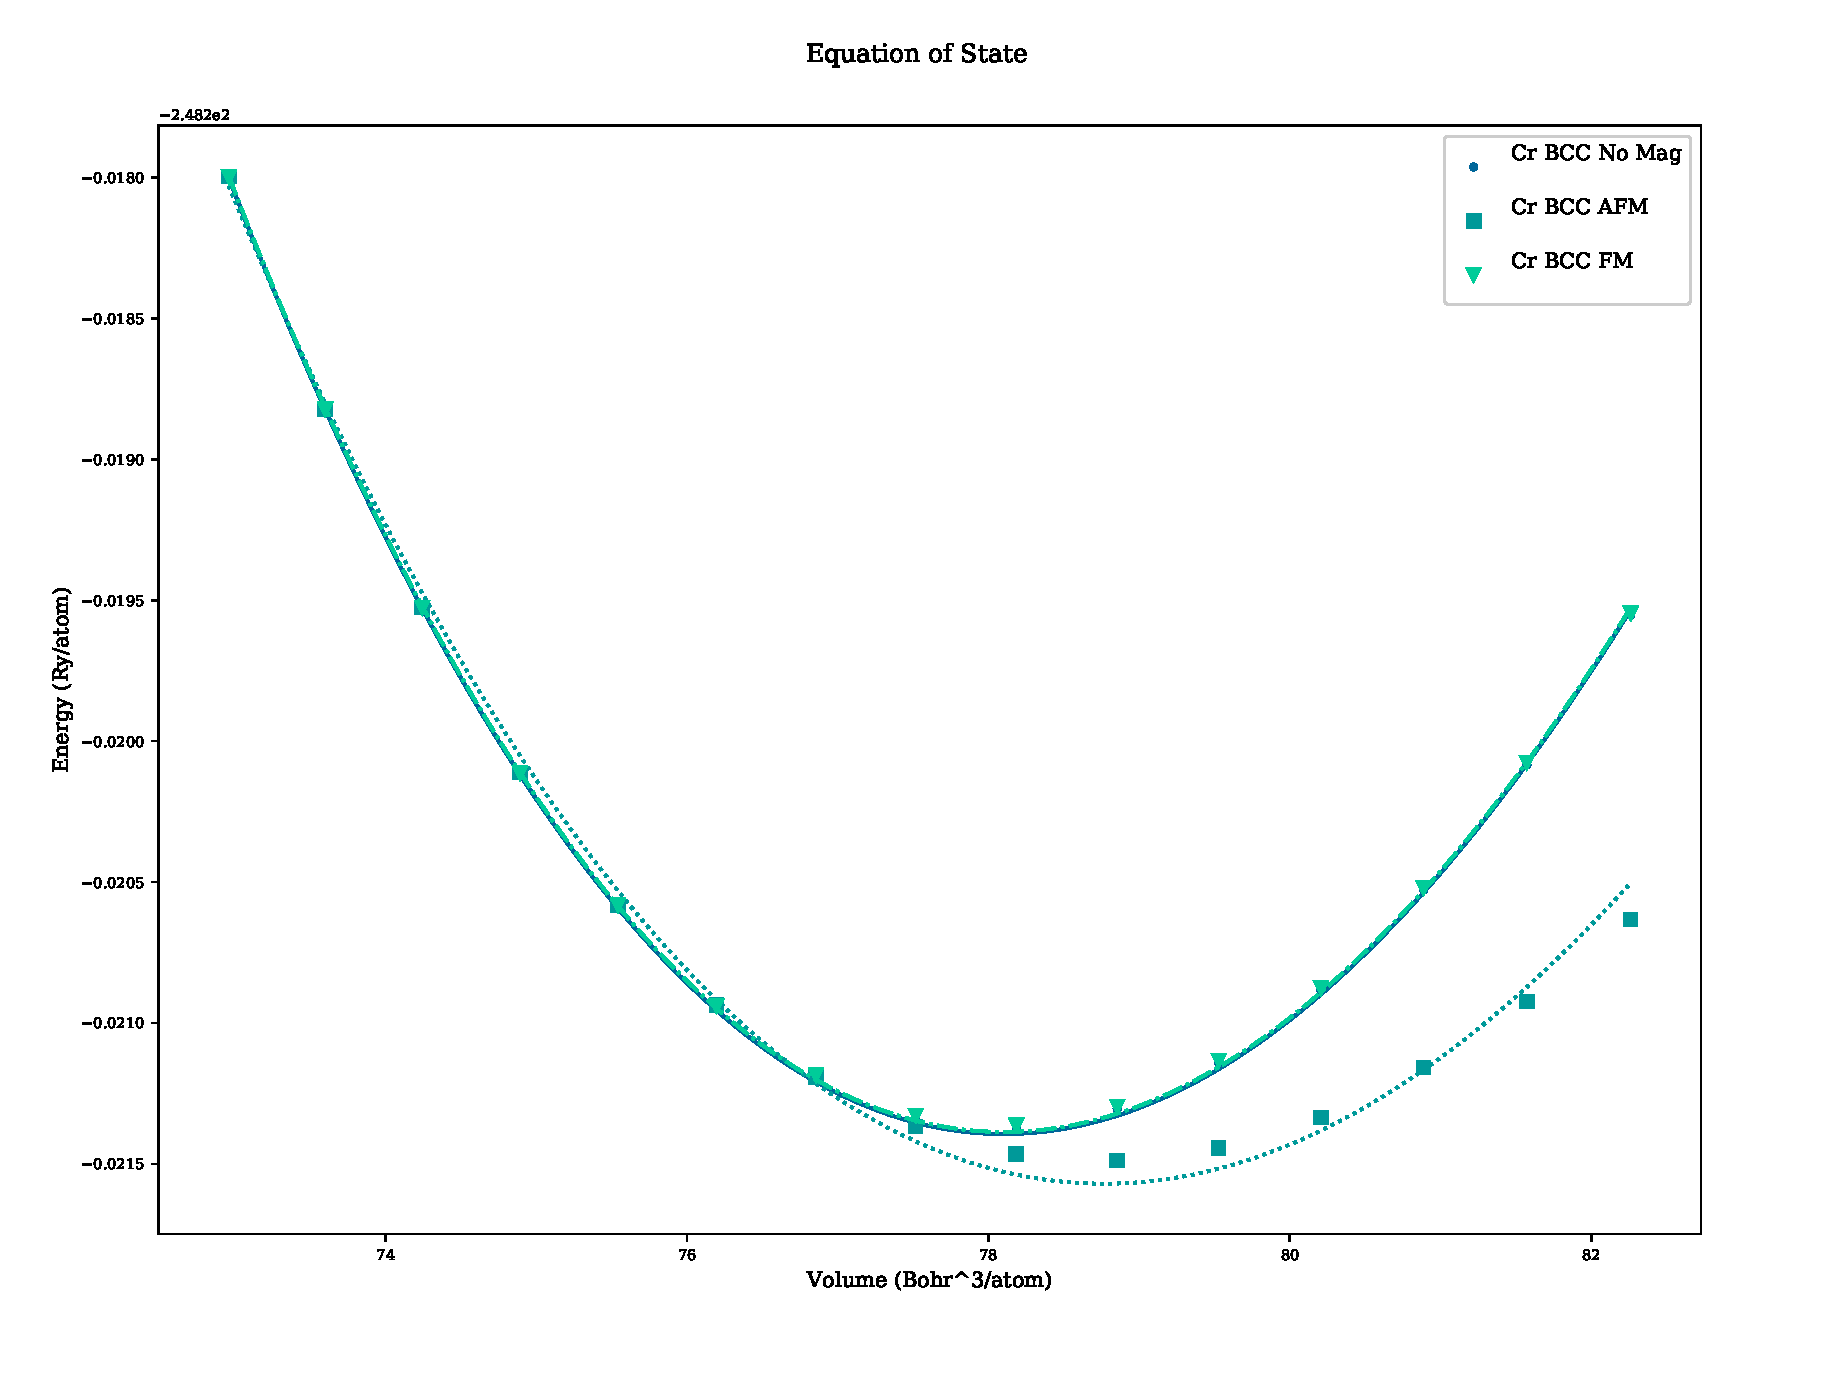
\includegraphics[scale=0.45]{chapters/potentials_fe_pd_ru/qeeos_plots/cr-mag/eos.eps}
\caption{Equation of state fit through data points for Chromium BCC with no magnetism, ferromagnetic and antiferromagnetic configurations}
\label{fig:chromiumeos}
\end{center}
\end{figure}


\FloatBarrier
\begin{table}[h]
\begin{center}
\renewcommand{\arraystretch}{1.2}
\begin{tabular}{c c c c c c}
\hline\hline
Description & $A_0$ (ang) & $V_0$ (bohr3) & $B_0$ (GPA) & $E_0$ (Ry) (DFT Only) \\
\hline\hline
Exp. & 2.91 & 83.23 & 160 & - \\
AFM & 2.86 & 78.77 & 217 & -248.2216 \\
FM & 2.85 & 78.10 & 267 & -248.2214 \\
No Mag & 2.85 & 78.102 & 267 & -248.2214 \\
\hline\hline
\end{tabular}
\end{center}
\caption{Chromium properties with and without collinear spin}
\label{table:crproperties}
\end{table}
\FloatBarrier

The equation of state was calculated for Chromium BCC in three ways: (1) with magnetism switched off, (2) atoms set in a ferromagnetic configuration (collinear, all in the same direction), (3) atoms set in an antiferromagnetic configuration (collinear, atoms in the same cell with spin in opposing directions).  

The DFT calculated values for the bulk modulus were larger than expected, but the antiferromagnetic calculation was much closer to the experimental value (table \ref{table:crproperties}).  The $E_0$ values do not reflect the actual energies, but show the relative calculated values.  The antiferromagnetic configuration gives the lowest, optimum, energy (fig. \ref{fig:chromiumeos}).

\FloatBarrier
\begin{figure}[h]
\begin{center}
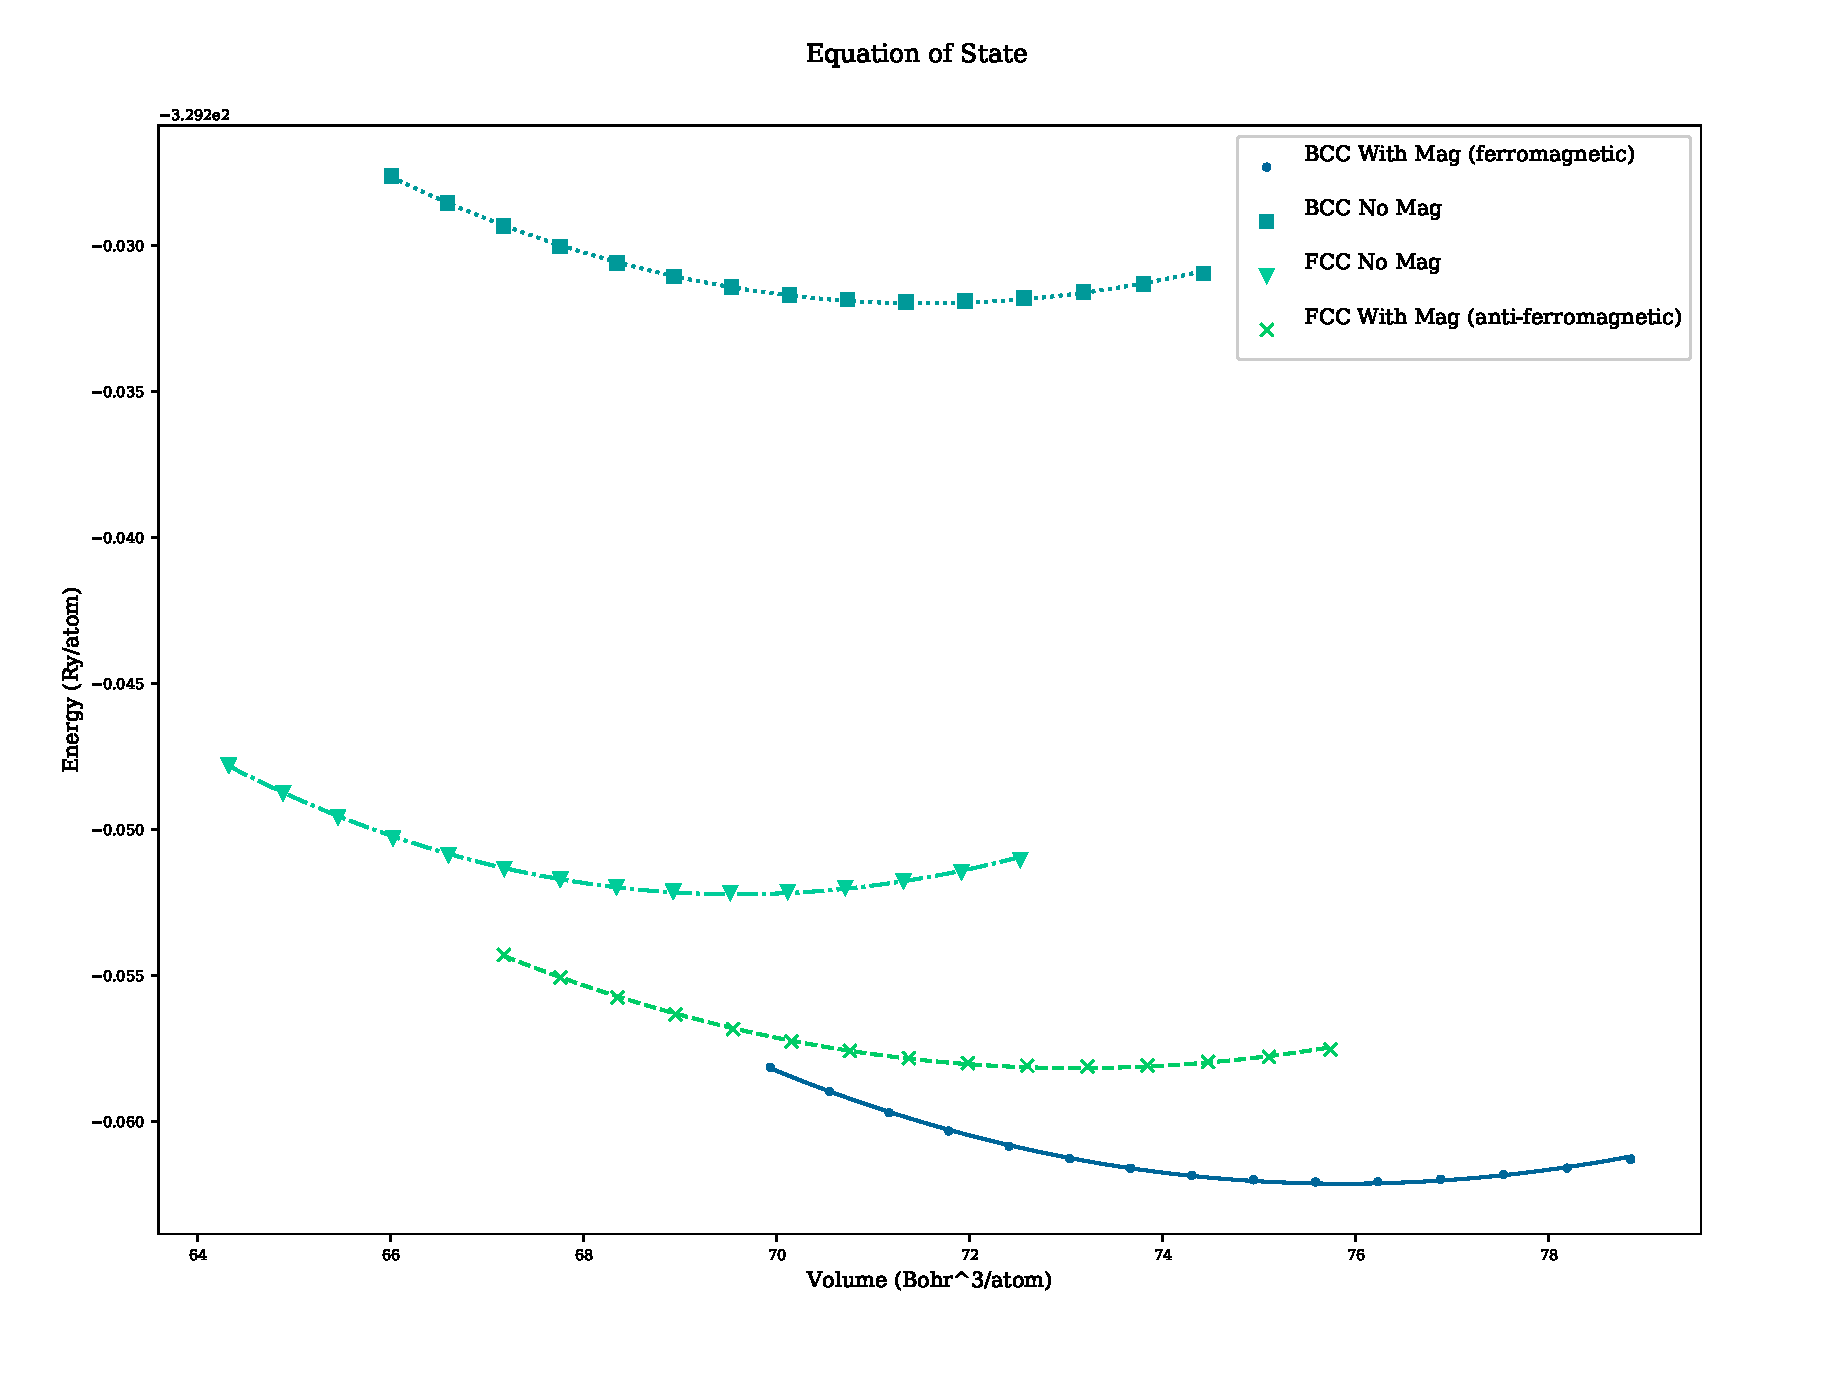
\includegraphics[scale=0.45]{chapters/potentials_fe_pd_ru/qeeos_plots/fe-mag/iron_eos_comparison.eps}
\caption{Equation of state fit through data points for Iron BCC (no magnetism, ferromagnetic) and Iron FCC (no magnetism and antiferromagnetic)}
\end{center}
\label{fig:iron_bcc_fcc_eos}
\end{figure}
\FloatBarrier


\begin{table}[h]
\begin{center}
\renewcommand{\arraystretch}{1.2}
\begin{tabular}{c c c c c c}
\hline\hline
Description & A0 (ang) & V0 ($bohr^3$) & B0 (GPA) & E0 (Ry) (DFT Only) \\
\hline\hline
Exp. & 2.86 & 79.01 & 170 & - \\
No Mag & 2.77 & 71.53 & 286 & -329.23 \\
FM & 2.82 & 75.9 & 239 & -329.26 \\
AFM & (failed) & (failed) & (failed) & (failed) \\
\hline\hline
\end{tabular}
\end{center}
\caption{\acrshort{bcc} Iron properties with and without collinear spin}
\label{table:feproperties}
\end{table}

In the case of Iron, both BCC and FCC configurations were used.  The antiferromagnetic configurations for both BCC and FCC failed in that the SCF calculations failed to converge.  As expected, the optimal configuration was BCC with ferromagnetism, and second to this was FCC with ferromagnetism.

Despite the increase in computational time, and other demands on resources such as scratch space and RAM per node, it was clear that collinear spin calculations were required for iron.  The lattice parameter value was within 2\% of the experimental value with the BCC structure set in a ferromagnetic state.  Whilst the bulk modulus is only within 41\% of the experimental value, this is an improvement over the non magnetic calculation that was almost 70\% away from the experimental bulk modulus (table \ref{table:feproperties}, figure \ref{fig:iron_bcc_fcc_eos}).


The QECONVERGE program was used to suggest the parameters to use, given the convergence threshold of $1.0 \time 10^{-5} RY/Bohr$ for forces and $1.0 \time 10^{-6} RY$ for energy.

\begin{table}[h]
\begin{center}
\renewcommand{\arraystretch}{1.2}
\begin{tabular}{c c c c c c c}
\hline\hline
Element & Pseudopotential & Ecutwfc & Ecutrho & K-points & Degauss & Atoms\\
\hline\hline
Al & Al PBE KJPAW & 50 & 200 & 11 & 0.04 & 32\\
Fe/Pd/Ru & PBE KJPAW & 71 & 431 & 9 & 0.04 & 32 \\ 
Fe/Pd/Ru & PBE KJPAW & 71 & 431 & Gamma & 0.04 & 128-256 \\ 
\hline\hline
\end{tabular}
\end{center}
\caption{DFT Settings - pseudo-potentials, ecutwfc, ecutrho, k-points, smearing}
\label{table:dftsettingsa}
\end{table}
\FloatBarrier

These settings in table \ref{table:dftsettingsa} were used throughout the remainder of the work.  The maximum values were selected from Fe, Ru and Pd as they were to be used for calculations of the pure elements and for binary allows of Fe-Ru and Fe-Pd.

The other settings used in PWscf throughout are listed in table \ref{table:dftsettingsb}.  Several of these values were arrived at by trial and error.  It was recommended by the authors of Quantum Espresso to adjust parameters such as the mixing beta if a calculation fails to converge.  The mixing mode was also changed from time to time, but overall the plain mode seemed to work best in most cases.

\begin{table}[h]
\begin{center}
\renewcommand{\arraystretch}{1.2}
\begin{tabular}{c c}
\hline\hline
Parameter & Value \\
\hline\hline
etot\_conv\_thr & 0.0001 \\
forc\_conv\_thr & 0.001 \\ 
conv\_thr & $1.0 \times 10^{-8}$ to $1.0 \times 10^{-6}$ \\ 
diagonalization & david \\ 
mixing\_beta & 0.1 to 0.3 \\ 
mixing\_mode & plain (local-TF for defects or randomised configurations) \\ 
\hline\hline
\end{tabular}
\end{center}
\caption{DFT Settings - other settings}
\label{table:dftsettingsb}
\end{table}

\FloatBarrier

The choices of parameters are supported by the convergence plots produced by the QECONVERGE code in figures \ref{image:aluminiumecut} and \ref{image:aluminiumkpointsmearing} (appendix \ref{section:dftconvplots}).













%%%%%%%%%%%%%%%%%%%%%%%%%%%%%%%%%%%%%%%%%%%%%%%%%%%%%%%%%%%%%%%%%%%%%%%%%%%%%%%%%%%%%%%%%%%%%%%%%%%%%%%%%%
%%
%%  QEEOS
%%
%%%%%%%%%%%%%%%%%%%%%%%%%%%%%%%%%%%%%%%%%%%%%%%%%%%%%%%%%%%%%%%%%%%%%%%%%%%%%%%%%%%%%%%%%%%%%%%%%%%%%%%%%%

\section{Bulk Property Calculations}

\subsection{QEEOS Python Program}
\label{section:qeeospyprog}

A Python code, QEEOS, (section \ref{code:qeeos}) has been developed to calculate bulk properties of a structure using the \acrshort{dft} code Quantum Espresso.  It is able to fit the equation of state for a cubic structure, and elastic constants for orthorhombic structures (which includes the subset of cubic structures).  In brief, the user provides a template PWscf input file, and the program adjusts the crystal basis vectors, applying the homogeneous strain and 9 distortions required to calculate the equation of state and elastic crystals, as discussed earlier in this work (section \ref{section:calcelasticconstants}).  The output data and highlights of this code are detailed in the results (section \ref{section:resultselastic}) and appendix (\ref{section:qeeosappendix}).


\subsection{DFT Calculations}

Although experimental data does exist for several of the structures, it was decided to calculate all the properties using \acrshort{dft}.  This was partly to confirm that both the QEEOS and PWscf, with the converged settings, were giving reasonable values and also to give data points that would better align with the energy, force and stress configuration calculations.

Experimental data is not available for \acrshort{fcc} Fe and \acrshort{fcc} Ru and so it was essential to compute these.  Although spin collinear equations were used throughout, it was particularly important for these settings to be used for Fe.  The relaxation step allowed for a relaxation of the atom positions, the basis vector and lattice parameter.  This gave cubic structures for Ru and Pd but a tetragonal structure for Fe.

The bulk property calculations were automated with the QEEOS code and this applied the preprogrammed nine strains, as discussed in section \ref{section:calcelasticconstants}, and the results are discussed in chapter \ref{chap:resultsdftdb}. 



%%%%%%%%%%%%%%%%%%%%%%%%%%%%%%%%%%%%%%%%%%%%%%%%%%%%%%%%%%%%%%%%%%%%%%%%%%%%%%%%%%%%%%%%%%%%%%%%%%%%%%%%%%
%%
%%  DFT Reference Database
%%
%%%%%%%%%%%%%%%%%%%%%%%%%%%%%%%%%%%%%%%%%%%%%%%%%%%%%%%%%%%%%%%%%%%%%%%%%%%%%%%%%%%%%%%%%%%%%%%%%%%%%%%%%%


\section{DFT Reference Database}

A database of configurations generated by \acrshort{dft} was compiled for Iron, Palladium, Ruthenium with alloys of Iron-Palladium and Iron-Ruthenium.  The potentials are derived for \acrshort{fcc} Iron and so these configurations were also \acrshort{fcc}.


\subsection{Bulk Property Calculations}

All the configurations in this work are \acrshort{fcc} structure crystals.  The QEEOS program (section \ref{section:qeeospyprog} and \ref{code:qeeos}) was used to compute the relaxed lattice parameter and primitive cell basis vector.

This program also automated the computation of equation of state, bulk modulus and elastic constants.  A 32 atom supercell was used for each pure element where the bulk properties were computed.  Ideally a large supercell or a larger number of k-points would have been used but throughout this work the number of processor cores per node ranged from 20-72 and this along with time constraints limits complexity of the calculations.

The data output from the QEEOS code forms a part of the reference database that is discussed in chapter \ref{chap:resultsdftdb}.



\subsection{Isolated Atom Settings}

\acrlong{dft} solves the Kohn-Sham equations for an infinite repeating lattice, and at first it doesn't seem applicable to single atoms or molecules that are not part of much larger lattice.  There are settings that may be used to compute the energy of an isolated atom and these are discussed on the Quantum Espresso forum\cite{qeforum} and Materials Square\cite{materialssquaresingleatom}. 

The settings of note used in these calculations were a configuration of just 1 isolated atom in a large cubic cell (20+ Bohr).  The computations were all nspin = 2 to ensure the electrons are computed spin up and down.  The assume\_isolated setting is given the makov-payne setting, as the system is a cube.

It was important to reduce the number of processor cores as too many would cause matrix decomposition errors for a low number of atoms, causing Quantum Espresso to crash.  An option to leverage more cores was to split the calculation into pools using the -npool input flag for PWscf, but this was not necessary for this set of calculations.




\subsection{Pure Element Defects}

The potentials are created to apply to \acrshort{fcc} Iron, Palladium, Ruthenium and alloys of Fe-Pd and Fe-Ru.  The configuration database will include several defects:

\begin{itemize}
\item octahedral interstitial
\item tetrahedral interstitial
\item 100, 110 and 111 interstitials
\item crowdion
\item a vacancy
\end{itemize}

The configurations for these defects were estimated using the perfect crystal positions of 2x2x2 supercells containing 32 atoms.  The defect or vacancy was applied, in some cases changing the total number of atoms, and the defect position was estimated.

A number of calculations, and the chance of a successful convergence in both the electronic state \acrshort{scf} calculation and relaxation calculation, were very sensitive on the input parameters.  Aluminium was not as sensitive and was used to relax the starting configuration.  This was then used as the starting point for either Fe, Pd or Ru.

Due to the periodic nature of these calculations, having only 32 atoms was not ideal as each defect cell would be very close to another.  Unfortunately, as stated a number of times, it was a constraint that was needed to be able to complete the work in a reasonable amount of time.

\FloatBarrier
\subsection{Alloy Atom Positions for Pd and Ru}

The stainless steel being studied is to be doped with 1\% or less of a \acrlong{pgm}.  Ideally a super cell with at least 256 atoms (4x4x4 primitive \acrshort{fcc} cells) would be used for all calculations, but due to the complexity of the calculations the majority were 2x2x2 super cells containing just 32 atoms.

\begin{figure}[htb]
\begin{subfigure}{.42\textwidth}
  \centering
  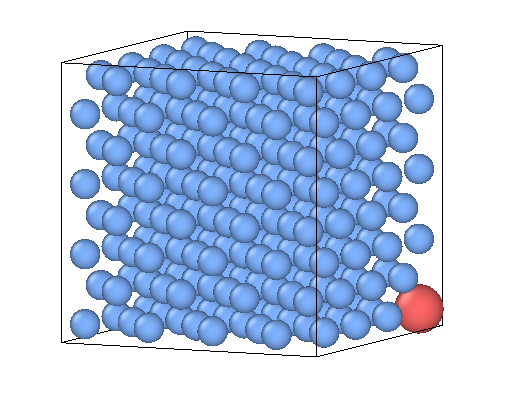
\includegraphics[width=.94\linewidth]{chapters/potentials_fe_pd_ru/slabs/bulk01.png}  
  \caption{Single atom, 256 atoms in total}
  \label{fig:sub-first}
\end{subfigure}
\begin{subfigure}{.42\textwidth}
  \centering
  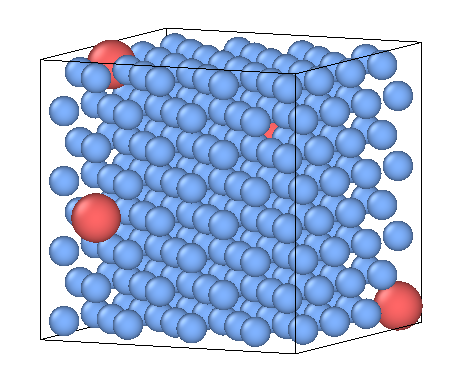
\includegraphics[width=.94\linewidth]{chapters/potentials_fe_pd_ru/slabs/bulk02.png}  
  \caption{Multiple atoms, 256 atoms in total}
  \label{fig:sub-first}
\end{subfigure}
\label{fig:binaryalloyconfigurationsbulk}
\end{figure}

Most of the configurations were prepared using the relaxed \acrshort{fct} structure computed for Fe.  One or more iron atoms were then replaced with either Pd or Ru.  The majority of calculations were carried out using the 32 atom configurations.  The larger 256 atom calculations were better suited to represent the low percentage of \acrshort{pgm} but were only computed using the gamma k-point (figure \ref{fig:binaryalloyconfigurationsbulk}).  This was another compromise in order to complete the calculations in time.



\subsection{Configurations with Randomised Positions}

Many of the atom configurations generated up to this point are symmetric and, whilst they have a variety of energies and stresses to use for fitting, the forces on the atoms are almost balanced and are small or none.  A large set of configurations with positions perturbed slightly from the exact lattice position are created.

Rather than use a linear random distribution a Gaussian distribution is used.  Some atoms had a larger perturbation but the majority are be slightly closer to the exact position, as would be expected with this type of distribution.  The maximum amount of perturbation was selected randomly between a minimum and maximum value.  

\begin{figure}[h]
\begin{center}
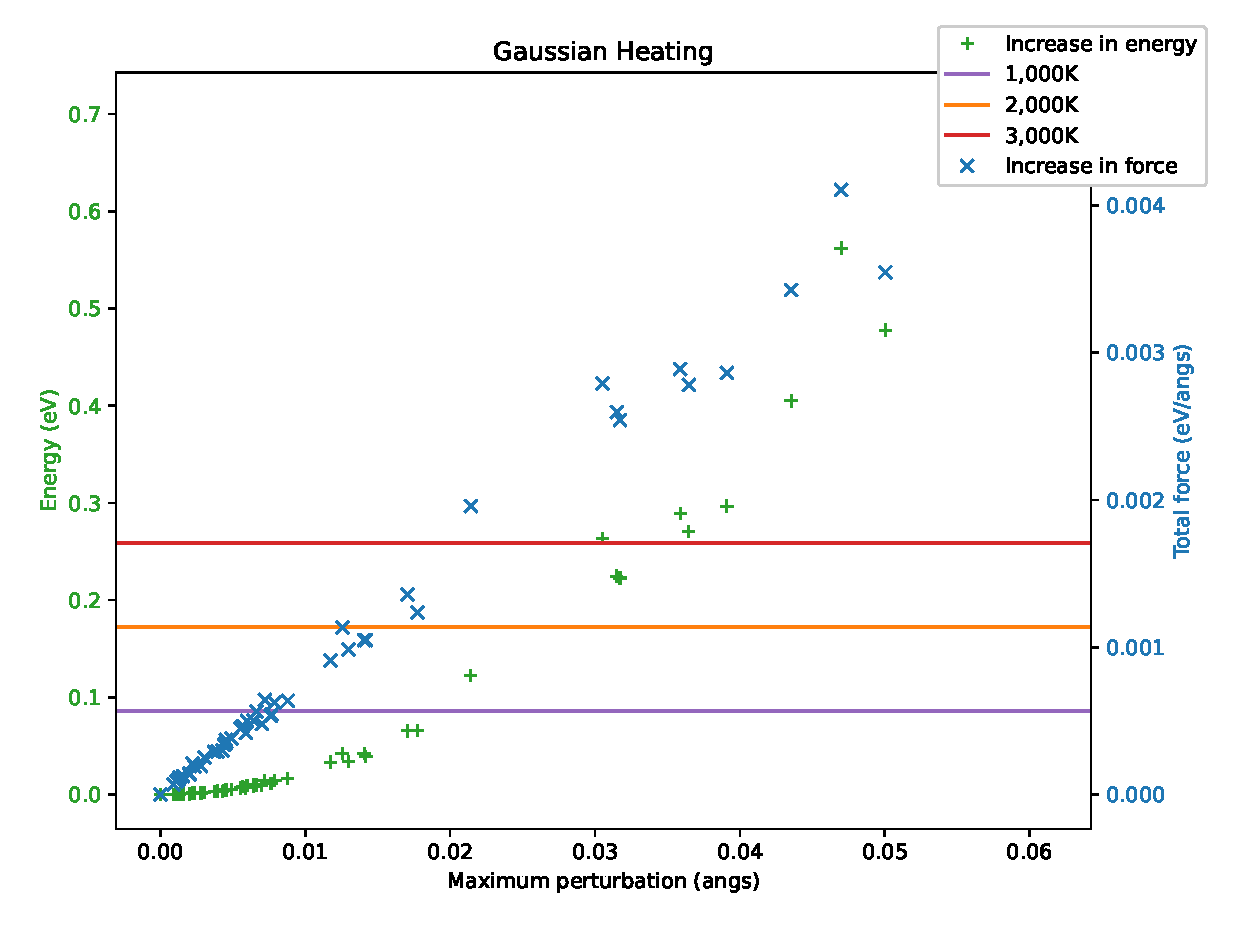
\includegraphics[scale=0.45]{chapters/potentials_fe_pd_ru/pwheat/al/alheat.eps}
\caption{Effect of randomly perturbing atom locations}
\label{fig:pwheatal}
\end{center}
\end{figure}

As the amount at which the atoms are perturbed increases, the energy and total force between the atoms increases.  If the disturbance increases too much, it will likely be useless for our needs as it would be beyond the temperatures relevant to this work, and it may also cause the \acrshort{scf} calculations to fail.

In the case of the alloy configurations, the randomised positions were loaded into the files.  In all cases convergence failed.  As perturbed atom positions had already been computed for Fe a new set of input files were created holding the Fe atoms in their perfect locations.  The added Pd and Ru atoms were then perturbed slightly from their perfect position within the lattice in order to compute forces and energies at slightly different positions.


\FloatBarrier
\subsection{Surface Energy Calculations}

One key aspect of this work is to determine whether or not either Pd or Ru are depleted from the surface at grain boundaries under irradiation.  With this in mind, the surface energies for the pure elements were calculated by creating a slab of atoms with an open surface on each side.

\begin{figure}[htb]
\begin{subfigure}{.32\textwidth}
  \centering
  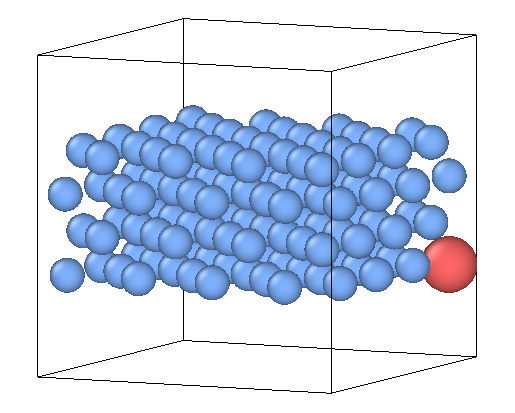
\includegraphics[width=.94\linewidth]{chapters/potentials_fe_pd_ru/slabs/slab01.png}  
  \caption{Single atom in the surface layer, 128 atoms in total}
  \label{fig:sub-first}
\end{subfigure}
\begin{subfigure}{.32\textwidth}
  \centering
  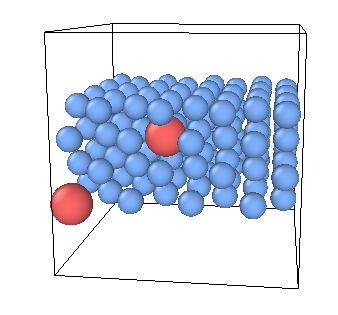
\includegraphics[width=.94\linewidth]{chapters/potentials_fe_pd_ru/slabs/slab02.png}  
  \caption{Single atom in bulk of slab, single atom in surface layer, 128 atoms in total}
  \label{fig:sub-first}
\end{subfigure}
\begin{subfigure}{.32\textwidth}
  \centering
  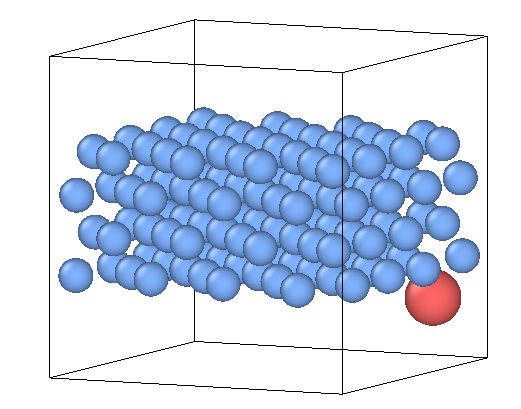
\includegraphics[width=.94\linewidth]{chapters/potentials_fe_pd_ru/slabs/slab03.png}  
  \caption{Single atom on the surface, 129 atoms in total}
  \label{fig:sub-first}
\end{subfigure}
\caption{A sample of configurations used for binary alloy \acrshort{dft} calculations for Fe-Pd and Fe-Ru.}
\label{fig:binaryalloyconfigurationsslab}
\end{figure}

A set of 32 atom configurations are used where the separation between the two facing surfaces is varied.  Several more 128 atom configurations are also prepared for the three pure elements.  To investigate the effect of a small addition of either Ru or Pd in the alloy a slab of Fe was prepared with Ru or Pd either within the slab, at the surface or on the surface (figure \ref{fig:binaryalloyconfigurationsslab}).  These examples were then added into the reference database used to fit the binary potentials.



\FloatBarrier
\subsection{Defects in Fe-Pd and Fe-Ru Alloys}

Attempts were made to compute simple defects in the alloy but the majority failed to converge, either in the electronic structure \acrshort{scf} iteration or a failure to relax geometrically that then lead to a \acrshort{scf} failure.  Rather than focus too much on this, more time was spent investigating Ru and Pd in a slab of Fe where the calculations were more successful.




%%%%%%%%%%%%%%%%%%%%%%%%%%%%%%%%%%%%%%%%%%%%%%%%%%%%%%%%%%%%%%%%%%%%%%%%%%%%%%%%%%%%%%%%%%%%%%%%%%%%%%%%%%
%%
%%  ERRORS
%%
%%%%%%%%%%%%%%%%%%%%%%%%%%%%%%%%%%%%%%%%%%%%%%%%%%%%%%%%%%%%%%%%%%%%%%%%%%%%%%%%%%%%%%%%%%%%%%%%%%%%%%%%%%


\section[Issues to Overcome]{DFT Errors, Convergence Failures and Repeat Calculations}

\subsection{Insufficient Memory}

The DFT calculations are performed on a supercomputer with many processors and many cores per processor.  The program uses two implementations of parallelization.

\begin{itemize}
\item OpenMP - many threads have access to the same shared memory
\item OpenMPI/MPICH - many processes, each with it's own memory
\end{itemize}

Whilst some favourable results have been shown using a hybrid of OpenMP and OpenMPI, it was more straightforward to use in OpenMPI mode only in this work.  Unfortunately, the amount of memory per process overwhelmed the computing nodes for certain calculation.  The job script was modified to reserve entire nodes and all the memory on each node, but to only use the cores on one of the two processors to halve the processes per node, but double the memory per process.  It was quicker to do this than wait in the high memory queue on BlueBEAR, where the memory per process would be perhaps double than that required.

\subsection{Scratch Restrictions}

When the calculations first started, the scratch space was located on a large shared space on the BlueBEAR computer.  Over time the drive space quota was restricted and the scratch was relocated to individual nodes.  There were few issues with less complex calculations as the \acrshort{scf} temporary data was several GB in size with the scratch space on each node being approximately 120GB.  Once a batch of collinear iron calculations had been submitted to the job queue, they would quickly fill the scratch drive and the job would terminate after just a few calculations, as the node had run out of scratch drive space.

\begin{lstlisting}[style=sPseudo,caption={Sbatch file},label={listing:sbatchfile}]
#!/bin/bash
#
#SBATCH --job-name=feforfit
#SBATCH --output=jobout.txt
#SBATCH --account=readmsd02
#
#SBATCH --ntasks 40
#SBATCH --nodes 1
#SBATCH --time 1800:00
#SBATCH --mem 180GB
#
#SBATCH --get-user-env
#SBATCH --export=NONE
#
unset SLURM_EXPORT_ENV

module purge; module load bluebear
module load bear-apps/2018a
module load iomkl/2018a
module load Python/3.6.3-iomkl-2018a
module load matplotlib/2.1.1-iomkl-2018a-Python-3.6.3

# Change to $PBS_O_WORKDIR
cd "$PBS_O_WORKDIR"
# Set the number of threads to 1
export OMP_NUM_THREADS=1
export PROC_COUNT=40
export PWSCF_SCRATCH=/scratch/bxp912
export PWSCF_PP=/rds/homes/b/bxp912/pp
export PWSCF_CACHE=/rds/homes/b/bxp912/pwscf_cache
export PWSCF_BIN=/rds/homes/b/bxp912/apps/qe-6.3/bin/pw.x
export PWSCF_SCRIPT=/rds/homes/b/bxp912/apps/qe-6.3/bin/pw.sh

python /rds/homes/b/bxp912/apps/python/qeforfit.py input.in > results.txt
\end{lstlisting}

\begin{lstlisting}[style=sPseudo,caption={Wrapper file},label={listing:wrapperfile}]
#!/bin/bash
rm -R $PWSCF_SCRATCH/*
mpirun -n $1 $PWSCF_BIN -in $2  > $3 
\end{lstlisting}

As the convergence and equation of state/elastic constant python programs automatically created and submitted the PWscf jobs, they would need to be continually restarted after clearing out the scratch.  To work around this a batch script (listing \ref{listing:sbatchfile}) and wrapper script (listing \ref{listing:wrapperfile}) for pw.sh were written.  The batch script sets the environment variables required for the sbatch job scheduling program and the wrapper script, and the wrapper script then clears the scratch directory before running PWscf.


\subsection{Caching Repeat Calculations}

Several of the programs required many hundreds of DFT calculations.  At first, if an error was encountered and the program had to start from scratch, computation time would be wasted.  To solve this, a directory was set to cache input and output files for PWscf.  A hash would be generated from the input file and this would be used as the cache file name.  If a calculation was successful, it would save the input and output file.  In future, if the same calculation was submitted again, the cached file would be returned.  The cache could be copied from BlueBEAR to other computers to save on repeat submission to the BlueBEAR job scheduler.


\subsection{Not Straying Too Far From Reality}

It is important to provide the calculation with reasonable and realistic configurations and settings.  Where a pure element such as Aluminium, Iron or Platinum was being investigated, the known experimental lattice parameters were used as a starting point (table \ref{table:predictedlattice} and table \ref{table:computedlattice}).  If the parameters were too far from these values, for example inputting a lattice parameter of either 2 or 8 angs for Aluminium rather than 4, as a starting approximation, the DFT calculation might struggle to relax the structure, or to even successfully run or converge a calculation.

The FCC Iron structure lattice parameter was estimated from the density of FCC steel, and the lattice parameter for alloys could similarly be estimated within a reasonable margin to use as a start point for the calculation.



\subsection{Adjustment of DFT Parameters}

Throughout the DFT segment of this work, there were a number of issues that either resulted in the calculations failing or completing and not converging.  There were a number of causes for this and several solutions were used throughout the process to converge the \acrshort{scf} calculation.

Where the ecutwfc and ecutrho parameters are not converged there is a danger that values too low therefore containing too few plane waves in the basis set.  This might cause problems with the \acrshort{scf} causing it not to converge.  The same can be said about a failure to pick appropriate k-points and smearing.

There are a selection of mixing modes available in PWscf, giving a choice of Thomas-Fermi screening for homogeneous systems, local density dependent Thomas Fermi (local-TF) screening for inhomogeneous screening and Broyden mixing as the default.  

\begin{figure}[htb]
\centering
\begin{subfigure}{.49\textwidth}
  \centering
  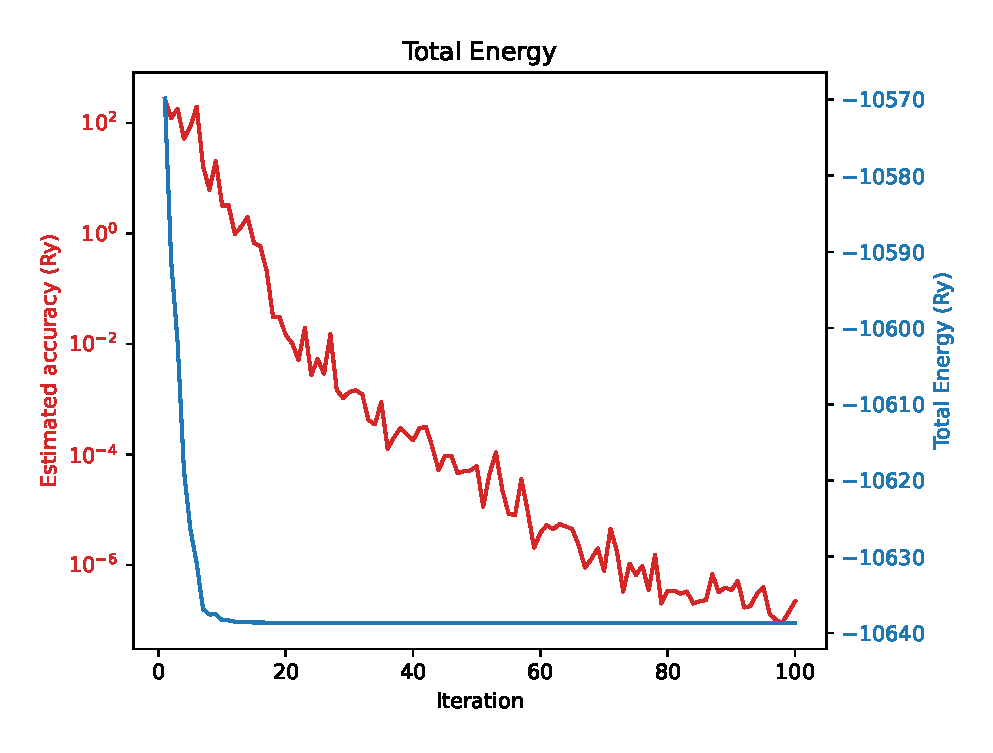
\includegraphics[width=.9\linewidth]{chapters/potentials_fe_pd_ru/convergence_failure/feru_1a_total_energy_0_plain.eps}
  \caption{Plain mixing failing to converge}
  \label{fig:feruplainmixing}
\end{subfigure}
\begin{subfigure}{.49\textwidth}
  \centering
  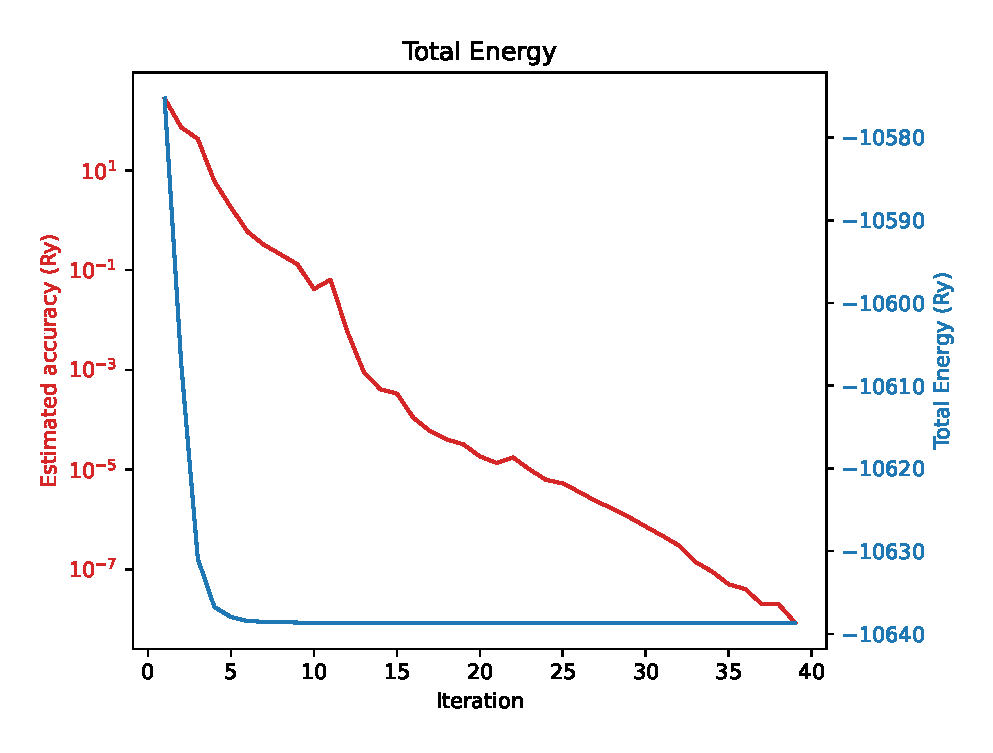
\includegraphics[width=.9\linewidth]{chapters/potentials_fe_pd_ru/convergence_failure/feru_1b_total_energy_0_local_tf.eps}
  \caption{Converging using local-TF mixing}
  \label{fig:ferulocaltfmixing}
\end{subfigure}
\caption{Fe-Ru calculations failed to converge in 100 iterations when plain mixing was used, but achieved convergence in under 40 iterations with local-TF convergence}
\label{fig:failuretoconverge}
\end{figure}

For calculations with defects the local-TF setting was used and for equation of state and elastic constant calculations, where the distribution of atoms is more homogeneous, plain Broyden mixing was used.  In most circumstances the mixing factor (mixing\_beta) was reduced to 0.1.  This wasn't always the case, and for certain defect calculations the default value of 0.3 proved to be the more efficient choice.

One other important parameter, that primarily affects geometry and position relaxation calculations (VC-RELAX), was the convergence threshold for the SCF calculations (conv\_thr).  The default value is $1.0\times 10^{-6}$ Ry and this was sufficient for SCF calculations and most VC-RELAX calculations.  Several relaxation calculations failed to converge and, at the suggestion of authors of Quantum Epresso, the threshold was reduced to $1.0\times 10^{-7}$ Ry.  This would lead to a longer time to compute the first geometry optimisation step.  As this result affects future steps the success of convergence for subsequent steps and the time taken to complete the optimisation was reduced. 



\subsection{Trial Parameters for Iron with and Octahedral Defect}

Calculations where there is a high level of symmetry finished relatively quickly and without much trouble.  Where the position of each atom was perturbed slightly or where there was a defect the \acrshort{scf} calculations would take more iterations to converge and would often fail completely.  Where the geometry and atom position was also being optimised through repeated sets of \acrshort{scf} iterations the calculation would begin to converge but would ultimately fail through \acrshort{scf} non convergence.

\begin{table}[h]
\begin{center}
\begin{tabular}{c c c c c c c c c}
\hline\hline
Nbnd & Ntype & K & Degauss & Scfconv & Beta & Ndim & Mode & Iterations \\
\hline\hline
317 & 5 & 9x9x9 & 0.04 & $1.0 \times 10^{-6}$ & 0.1 & 10 & Plain & 75 \\
320 & 3 & 9x9x9 & 0.04 & $1.0 \times 10^{-6}$ & 0.05 & 10 & Local-TF & 46 \\
317 & 3 & 9x9x9 & 0.04 & $1.0 \times 10^{-7}$ & 0.1 & 10 & Local-TF & 42 \\
340 & 3 & 9x9x9 & 0.04 & $1.0 \times 10^{-6}$ & 0.8 & 8 & Local-TF & 38 \\
320 & 3 & 9x9x9 & 0.04 & $1.0 \times 10^{-6}$ & 0.1 & 10 & Local-TF & 36 \\
317 & 3 & 9x9x9 & 0.04 & $1.0 \times 10^{-6}$ & 0.8 & 8 & Local-TF & 33 \\
317 & 5 & 9x9x9 & 0.04 & $1.0 \times 10^{-6}$ & 0.3 & 8 & Local-TF & 32 \\
317 & 3 & 9x9x9 & 0.04 & $1.0 \times 10^{-6}$ & 0.3 & 8 & Local-TF & 32 \\
320 & 3 & 9x9x9 & 0.04 & $1.0 \times 10^{-6}$ & 0.3 & 10 & Local-TF & 29 \\
320 & 3 & 11x11x11 & 0.04 & $1.0 \times 10^{-6}$ & 0.3 & 10 & Local-TF & 29 \\
320 & 3 & 13x13x13 & 0.04 & $1.0 \times 10^{-6}$ & 0.3 & 10 & Local-TF & 29 \\
320 & 3 & 9x9x9 & 0.07 & $1.0 \times 10^{-6}$ & 0.3 & 10 & Local-TF & 25 \\
\hline\hline
\end{tabular}
\end{center}
\caption{Improving convergence SCF calculations of defects in Iron}
\label{table:trialparametersocta}
\end{table}

Iron with an octahedral defect was used to help fine tune parameters.  Initially a set of \acrshort{scf} calculations were performed with different parameters, and finally these were used to relax the cell geometry and atom positions for this defect.

Changing the number of k-points did not have an impact on the number of iterations required to converge, but changing the smearing value did.  An increase in smearing would be detrimental to the accuracy of convergence to the correct value and by doing this it would cause a difference in energy between past calculations with a smearing of 0.04Ry and and those with 0.07Ry.

The adjustment that had the largest impact on reducing the number of iterations was the change from plain mixing to Local-TF.  Following this, using a mixing beta of 0.3 where more weight is given to the previous state, also helped to reduce the number of iterations.

The attempts to optimise the values was not exhaustive as there were constrictions on time.  However, despite making these improvements and reducing the convergence threshold to $1.0 \times 10^{-8}$, the cell geometry and position relaxation of the starting configuration for an octahedral defect (by adding an atom at the octahedral location) also fails to relax by \acrshort{scf} non-convergence within an iteration of the relaxation algorithm. 

The optimization of the geometry and atom positions was likely due to it being a complex system to model with the initial configuration too far from the relaxed one.  To work around this the octahedral defect for a more simple metal, Aluminium, was relaxed to give a better starting point for the Iron calculation.  The increase in cell size was also applied.  With a better initial configuration and the adjusted parameters, the Iron octahedral calculation successfully completed.

This process was repeated for tetrahedral, 100, 110, 111 and crowdion defects.






%%%%%%%%%%%%%%%%%%%%%%%%%%%%%%%%%%%%%%%%%%%%%%%%%%%%%%%%%%%%%%%%%%%%%%%%%%%%%%%%%%%%%%%%%%%%%%%%%%%%%%%%%%
%%
%%  EAMPA: Potential Analysis and Fitting Code
%%
%%%%%%%%%%%%%%%%%%%%%%%%%%%%%%%%%%%%%%%%%%%%%%%%%%%%%%%%%%%%%%%%%%%%%%%%%%%%%%%%%%%%%%%%%%%%%%%%%%%%%%%%%%


\section[EAMPA]{EAMPA: Potential Analysis and Fitting Code}

A python-fortran based computer code was developed to fit interatomic potentials to bulk properties and DFT calculated forces and energies.  It has been designed to take advantage of both Fortran and Python.  Fortran is used to compute the neighbour lists, energies, stresses and forces, and Python is used to read and write data, produce plots and control the potential fitting.  This allows the use of custom optimization subroutines as well as the use of those included in the SciPy module.  Highlights from the code are discussed in the results (section \ref{code:eampa}) and the appendix of this work (appendix \ref{chapter:appendix-eampa}).





%%%%%%%%%%%%%%%%%%%%%%%%%%%%%%%%%%%%%%%%%%%%%%%%%%%%%%%%%%%%%%%%%%%%%%%%%%%%%%%%%%%%%%%%%%%%%%%%%%%%%%%%%%
%%
%%  Palladium and Iron Potentials
%%
%%%%%%%%%%%%%%%%%%%%%%%%%%%%%%%%%%%%%%%%%%%%%%%%%%%%%%%%%%%%%%%%%%%%%%%%%%%%%%%%%%%%%%%%%%%%%%%%%%%%%%%%%%



\section[Potential Transferability]{Investigating the Transferability of Existing Potentials}

There are currently a number of \acrshort{eam} Iron potentials, as well as a \acrshort{meam} potential for Fe-Pd.  Several pure element potentials also exist for Ruthenium and Palladium.  Whilst it would be convenient to have a one size fits all potential, this is not the case.  Taking the Ruthenium potential as an example, in work that required the reproduction of stacking fault and surface energy of the element, the existing potentials were inadequate and a new potential was developed\cite{mendelevruau}.

Several potentials were selected to test transferability.  First, the FCC Sheng potential for Aluminium was applied to both FCC and BCC structures in the EAMPA code.  The properties of FCC Aluminium are known, and those for BCC Aluminium were calculated using DFT.  This investigation shows that some properties, such as the lattice constant, does transfer quite well to the new structure, but the bulk modulus and $C_{11}$ elastic constant are both poorly reproduced (table \ref{table:alshengtransferability}).  

\begin{table}[h]
\begin{center}
\begin{tabular}{c c c c c}
\hline\hline
Property   & Al FCC Exp. & Al FCC Sheng &  Al BCC DFT & Al BCC Sheng \\
\hline\hline
a0             & 4.05  &  4.02        & 3.23     & 3.18     \\
e0             & -3.36 & -3.36        & -3.26    & -3.27    \\
b0             & 76    &  86          & 69       & 50       \\
$C_{11}$       & 114   &  124 (125)   & 47 (47)  & 11 (5)   \\
$C_{12}$       & 62    &  67 (66)     & 81 (24)  & 70 (63)  \\
$C_{44}$       & 32    &  29 (32)     & 40 (12)  & 29 (42)  \\
\hline\hline
\end{tabular}
\end{center}
\caption{Applying the Sheng Al potential, developed for FCC crystals, to the BCC structure.  Elastic constants are calculated using the method by Mehl et al with values from the method by Ravindran et al in brackets.}
\label{table:alshengtransferability}
\end{table}

The Mendelev 2003 potential was developed to fit the properties of BCC Iron, but also to reproduce the transition from BCC to FCC at high temperatures.  However, when using this potential for low  temperature FCC Iron, it does not reproduce the properties predicted by DFT.  All 9 orthorhombic elastic constants have been omitted in table \ref{table:femendelevtransferability}, but there is a significant difference for the three elastic constants given as well as the bulk modulus.

\begin{table}[h]
\begin{center}
\begin{tabular}{c c c c c}
\hline\hline
Property   & Fe BCC Exp. & Fe BCC Mendelev &  Fe FCC DFT & Fe FCC Mendelev \\
\hline\hline
a0             &   2.86  &   2.86      &   3.42   &   3.59          \\
e0             &  -4.32  &  -4.13      &  -4.26   &  -4.01          \\
b0             &   170  &    176       &  226     &   98            \\
$C_{11}$       &   243  &   255 (260)  &  364     &   6 (79)        \\
$C_{12}$       &   145  &   137 (143)  &  142     &   145 (69)      \\
$C_{44}$       &   116  &   114 (111)  &  186     &   86 (48)       \\
\hline\hline
\end{tabular}
\end{center}
\caption{Applying the Sheng Al potential, developed for FCC crystals, to the BCC structure.  Elastic constants are calculated using the method by Mehl et al with values from the method by Ravindran et al in brackets.}
\label{table:femendelevtransferability}
\end{table}

Finally the Ackland 1997 potential for Iron was tested.  This older potential gives a better value for the cohesive energy when transferred to the FCC structure, but other properties such as the relaxed lattice constant are quite different (table \ref{table:feacklandtransferability}).

\begin{table}[h]
\begin{center}
\begin{tabular}{c c c c c}
\hline\hline
Property   & Fe BCC Exp. & Fe BCC Mendelev &  Fe FCC DFT & Fe FCC Mendelev \\
\hline\hline
a0             &   2.86  &   2.87      &   3.42   &   3.62          \\
e0             &  -4.32  &  -4.32      &  -4.26   &  -4.26          \\
b0             &   170  &    200       &  226     &   141            \\
$C_{11}$       &   243  &   265 (248)  &  364     &   117 (140)        \\
$C_{12}$       &   145  &   168 (151)  &  142     &   153 (117)      \\
$C_{44}$       &   116  &   125 (128)  &  186     &   164 (94)       \\
\hline\hline
\end{tabular}
\end{center}
\caption{Applying the Sheng Al potential, developed for FCC crystals, to the BCC structure.  Elastic constants are calculated using the method by Mehl et al with values from the method by Ravindran et al in brackets.}
\label{table:feacklandtransferability}
\end{table}

This investigation into existing potentials shows that whilst some of the properties are replicated, many do not match the DFT computed values.  This supports the derivation of new potentials to be fit that replicate the DFT values and take into account the characteristics of a number of provided configurations.  Additional plots are included in the appendix that show the expected equations of state compared to those generated using the above potentials (section \ref{section:transferabilityappendix}).




\section{Fitting Potentials with EAMPA}

The custom computer code EAMPA was developed in order to fit the parameters for the potentials to the \acrshort{dft} reference database.  It was a long process that utilised nodes on the University of Birmingham BlueBEAR computer.  At the time of writing, the code was able to fit energy, forces and bulk properties.  I was not convinced that the computation of stress in EAMPA and in PWscf were identical and so throughout I set the weighting of stress to zero.

\subsection{Choice of Function and Functional}

A number of functions and functionals have been used previously and these are discussed in detail in chapter \ref{chap:backgroundfitting}.  Several were used to attempt to fit the potentials, but eventually the cubic splines and tight binding type functional, as used by Mendelev, Ackland, Bonny et al, were selected.

Initially, I looked to the computer program DIRAC for the density function, as it computes the radial electron density distribution (figure \ref{fig:dirac-fe-density-plot} and figure \ref{fig:dirac-fe-density-plot}).  Unfortunately, as may be expected, there were a number of issues in using the density distribution of a single atom.  The atomic separation for both iron and palladium, for a relaxed crystal, begins at approximately 2-2.5 angstrom, but most of the electrons, from all shells, are distributed much closer.  The plot does not take into consideration the valence electrons shared in the crystal, bonding the metal atoms together.

From the point of view of the potential, the pair potential will dominate at small separations due to the \acrshort{zbl} function.  The density function will be important at separations of 2 angstrom up to the cutoff radius (5-6 angstrom).  For this reason, the idea to use the DIRAC computed densities was abandoned in favour of a cubic spline.

\begin{figure}[htb]
\minipage{0.49\textwidth}
	\begin{center}
  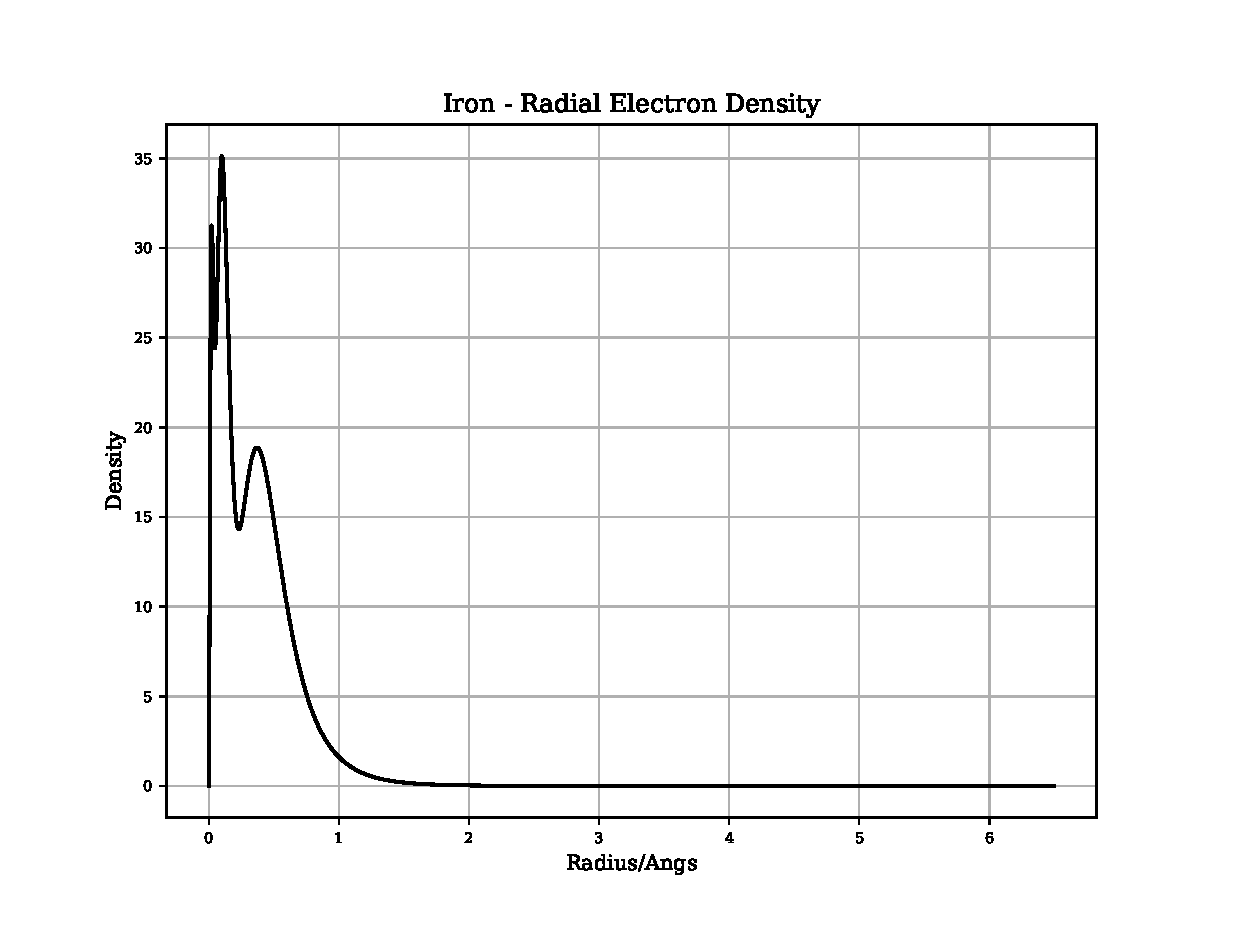
\includegraphics[width=0.9\linewidth]{chapters/potentials_fe_pd_ru/density/fe.eps}
  \captionsetup{font={it}}
  \caption{DIRAC calculated radial electron density for Iron}
  \label{fig:dirac-fe-density-plot}
	\end{center}
\endminipage\hfill
\minipage{0.49\textwidth}
	\begin{center}
  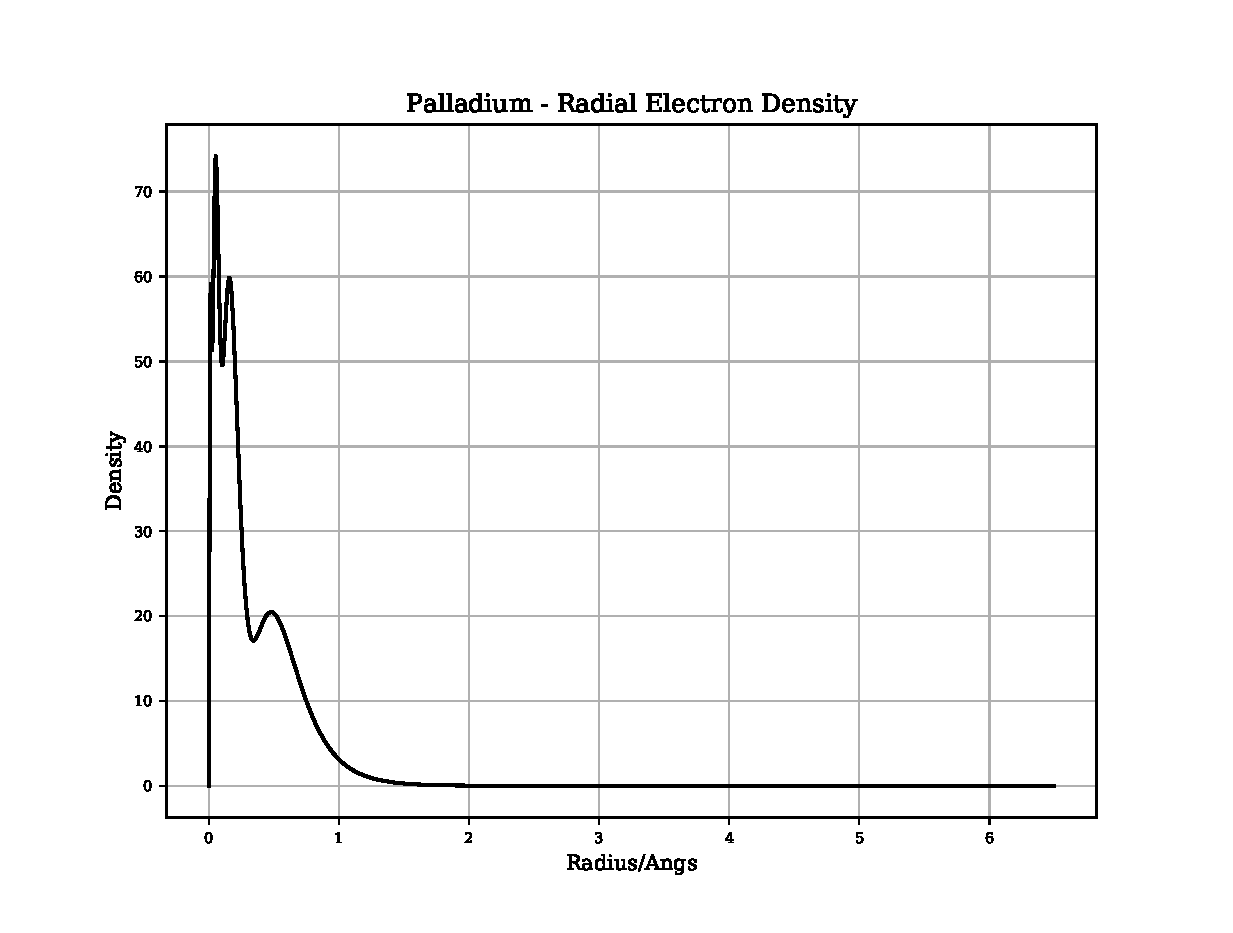
\includegraphics[width=0.9\linewidth]{chapters/potentials_fe_pd_ru/density/pd.eps}
  \captionsetup{font={it}}
  \caption{DIRAC calculated radial electron density for Palladium}
  \label{fig:dirac-pd-density-plot}
	\end{center}
\endminipage
\end{figure}

One interesting feature that Bonny used in his code was to add a hard core spline to the pair potential with a positive coefficient.  This was to ensure that at small separations, say below 1.5-1.8 angstrom, the atoms would repel.  The cubic spline used in this work for the density also has a fixed positive coefficient to help stop negative densities for small separations.  This is dependent on the number of cubic splines used, and is a feature that can be turned off in the EAMPA code.

A cubic spline was also used for the pair potential, and as with Bonny's code, this had a hard core potential but in addition to this a \acrshort{zbl} core was added to the entire potential to ensure the exponential increase in energy as modelled with the \acrshort{zbl} function.  This was to ensure the potential would both model the material when out of a radiation field, where the atoms are several angstrom apart, but also able to capture a damage cascade where the separation drops and the \acrshort{zbl} becomes the dominant feature, over both the pair cubic spline and the embedding functional.

There was a choice of several embedding functionals but one based on the Finnis-Sinclair and \acrshort{eam} was used.  It consisted of the square root term but also a zeroth power and square term for greater flexibility.  The addition of a fourth power term had been trailed, but occasionally when fitting the parameters the coefficient of the fourth power would become negative leading to a negative energy at high electron densities.


\subsection{Searching Parameter Space}

Improving the potential was an iterative process that required multiple runs of EAMPA feeding the last potential as a starting point for the next potential.  In the first instance, the exact bulk property fitting code of Bonny was used, but it did not always find the parameters that reproduced the data points it was given.  This was perhaps due to a lack of data and knowledge on how to use the code effectively, but it did give a starting point with a modest number of cubic splines for the density and pair functions.

These initial set of parameters were then used with EAMPA.  The first task with this code was to find parameters that replicated the energies, forces and bulk properties for each of the pure elements.

The type of search could be adjusted for each fitting job, but the typical process was as follows.  A short random search through parameter space followed by a small simulated annealing search with a wide search area.  This was then followed by a genetic algorithm search with quite a wide search area.  Next a second genetic algorithm search over a smaller range of parameters but with more iterations and a larger population, and this step used most of the computation time.  Finally a short simulated annealing and local \acrshort{bfgs} minimizer were used before outputting optimised parameters.  A sample input is given in listing \ref{lst:searchsettings}, but the user is free to add fewer or more steps and search types.

\begin{lstlisting}[style=sEmail,caption={Parameter search settings when fitting in EAMPA}, label={lst:searchsettings}]
#FIT type=RAND niter=1000 
#FIT type=SA niter=1000 titer=10 tstart=100.0 tend=0.001 pfact=0.5 pvar=10.0 vartype=add gaussian=True
#FIT type=GA niter=200 popsize=500 fresh=0.2 search=w
#FIT type=GA niter=5000 popsize=2000 fresh=0.2 search=n
#FIT type=SA niter=1000 titer=15 tstart=1.0 tend=0.001 pfact=0.5 pvar=0.01 vartype=add gaussian=True
#FIT type=BFGS
\end{lstlisting}

The code has an option to set the random seed such that every job with that seed and settings will return the same output.  This allowed ten or more jobs to be run in parallel, with 4 cores per job, and a different seed for each job.  Typical run times were 3-5 days per iteration and several iterations required.

At the start of the fitting process all available configurations were used, but it turned out to be difficult for the code to satisfy all the constraints given the simplicity of the \acrshort{eam} potentials.  Towards the end of the process many of the configurations were removed with bulk and surface/slab configurations being left.  This was in order to train the potential specifically to these configurations in favour of the entire set.  

Once the pure potentials for Fe, Pd and Ru were determined, they each underwent an effective gauge transform, with the transform being that used by Bonny et al\cite{bonnyfecr}\cite{bonnymalerba}.  Due to this transform, they were converted from analytic potentials to numeric.  

The fixed numeric functions were then used in the binary alloy fitting where the only parameters adjusted are those for the cross pair potential.  The searching method was similar to that used for the pure elements, but the configurations were changed to those containing both species of atom.  The bulk property fitting was also removed as this fitting was only applicable to the pure elements.



\section{DL\_POLY Contribution}

DL\_POLY is a Molecular Dynamics code developed by W. Smith, T.R. Forester and I.T. Todorov at Daresbury Laboratory in Warrington. It is written in Fortran and, before the modifications, included a number of potential types for metals including:

\begin{itemize}
\item Finnis Sinclair
\item EAM
\item EEAM
\end{itemize}

The Finnis Sinclair is a particular form of the EAM potential, and EEAM is a modification where, is the metal is an alloy, the density and embedding functional for each atom type are treated separately.

A meeting was held with Dr. Todorov at Daresbury Laboratory, where a brief overview of the relevant code was given.  After this point, and corresponding by email, the two band EAM type was added (2BEAM).  The code was altered with the addition of an array used to store the d-band density function and d-band embedding functional, with the s-band function/functional using the original density function and embedding functional arrays.  The calculation of energy and forces on atoms was also altered to make use of these arrays where a \acrlong{2beam} potential is used.

\begin{lstlisting}[style=sEmail,caption={DL\_POLY 4.05 mailshot extract}]
DL_POLY_4.05: New Release & Events - MAILSHOT 013

NEW FEATURES \& IMPROVEMENTS
--------------------------- 
1.  New two band (2B) EAM and EEAM potentials for metals (TEST45 and TEST46). 

Acknowledgements
----------------
Ben Palmer \@ University of Birmingham (UK) for contributing to the
development and testing of the 2BEAM for metals;

Regards,

Ilian Todorov
July 2013 


\end{lstlisting}

Extracts of the modified DL\_POLY code are included in appendix \ref{chapter:appendixdlpoly}.





























%%%%%%%%%%%%%%%%%%%%%%%%%%%%%%%%%%%%%%%%%%%%%%%%%%%%%%%%%%%%%%%%%%%%%%%%%%%%%%%%%%%%%%%%%%%%%%%%%%%%%%%%%%
%%
%%  Convergence Results
%%  
%%%%%%%%%%%%%%%%%%%%%%%%%%%%%%%%%%%%%%%%%%%%%%%%%%%%%%%%%%%%%%%%%%%%%%%%%%%%%%%%%%%%%%%%%%%%%%%%%%%%%%%%%%


















%%%%%%%%%%%%%%%%%%%%%%%%%%%%%%%%%%%%%%%%%%%%%%%%%%%%%%%%%%%%%%%%%%%%%%%%%%%%%%%%%%%%%%%%%%%%%%%%%%%%%%%%%%
%%
%%  Preliminary Calculations
%%  
%%%%%%%%%%%%%%%%%%%%%%%%%%%%%%%%%%%%%%%%%%%%%%%%%%%%%%%%%%%%%%%%%%%%%%%%%%%%%%%%%%%%%%%%%%%%%%%%%%%%%%%%%%


\FloatBarrier
\section{Preliminary Calculations}

\subsection{Relaxed Crystal Calculations}

The cohesive energy is an important value in relation to the interatomic potential.  The energies calculated by \acrshort{dft} code depend on many factors including the energy under which plane-wave are cut-off, the degauss value, k-point settings and the \acrshort{scf} convergence parameters.  What is more important in the \acrshort{dft} calculations is the difference in energy between calculations.  As the cohesive energy is known, a \acrshort{dft} calculation may be performed for each species of atom to determine the relaxed energy.  This value may then be used to calibrate other \acrshort{dft} calculations, so they are given relative to the energy of each atom spaced infinitely far from one another, with a binding energy of 0eV.  The relaxed energies, the settings used to calculate them and the adjustment to convert them to the \enquote{real} energies are given in table \ref{table:relaxedenergies}.

\clearpage
\begin{landscape}

\begin{table}[h]
\begin{center}
\renewcommand{\arraystretch}{1.2}
\begin{tabular}{c c c c c c c}
\hline\hline
Measurement & Al FCC & Fe BCC & Fe FCC & Pd FCC & Ru HCP \\
\hline\hline
Element                    & Aluminium & Iron & Iron & Palladium & Ruthenium & Ruthenium \\
Structure                  & FCC  & BCC  & FCC  & FCC  & HCP  & FCC     \\
Ecutwfc (Ry)               & 50  & 71  & 71  & 71  & 71  & 71    \\
Ecutrho                    & 200 & 430  & 430  & 430 & 430  & 430   \\
K-points                   & 11 11 11 & 9 9 9  & 9 9 9  &  9 9 9  &  9 9 9  &  9 9 9  \\ 
Smearing (Ry)              & 0.04  & 0.04  & 0.04  & 0.04 & 0.04 & 0.04   \\ 
NSpin                      & 0 & 2  & 2  & 0 & 0 & 0  \\ 
Starting Magnetism         & None & FM  & AFM  & None  & None  & None   \\ 
No. Atoms                  & 32  & 16  & 32  & 32 & 16 & 32  \\  
Energy (Ry)                & -1264.08749654  & -5268.18846365   & -10536.25040753    & -16384.95803030  & -6906.78722345  & -13813.30088106  \\
Energy/Atom (Ry)           & -39.502734267   & -329.261778978   & -329.257825235     & -512.029938447 & -431.674201466 & -431.665652533  \\
Energy/Atom (eV)           & -537.462275214  & -4479.836349416  & -4479.782555982    & -6966.524743211   \\
Known Cohesive Energy (eV) & -3.36           & -4.316           & -4.26 (Calculated) & -3.91  & -6.74  & -6.62 (Calculated)             \\
Adjustment/atom (eV)       &  534.102275214  &  4475.520349416  &  4475.520349416    &  6962.614743211 & 5866.47338  &  5866.47338 \\
Relaxed $a_0$ (Bohr)       & 15.265          & 10.594           & 12.937             & 14.845            \\
Relaxed $c$ (Bohr)       & None  & None  & None  & None  & 1.5773  & None \\
$U_{xx}$                   & 1.000           & 1.000            & 1.000              & 1.000              & 1.000            & 1.000           \\
$U_{yy}$                   & 1.000           & 1.000            & 1.054              & 1.000               & 0.8660            & 1.000          \\
$U_{zz}$                   & 1.000           & 1.000            & 1.000              & 1.000                & 1.5773            & 1.000         \\
$U_{yx}$                   & 0.000           & 0.000            & 0.000              & 0.000                & -0.5            & 0.000         \\
\hline\hline
\end{tabular}
\end{center}
\caption{Relaxed energies calculated in Quantum Espresso}
\label{table:relaxedenergies}
\end{table}

\end{landscape}
\clearpage




\subsection{Relaxed FCC Iron}
\label{section:fcc-iron}

The configuration for Fe has been referred to throughout this work as \acrshort{fcc}, but the relaxed collinear spin-polarized \acrshort{dft} calculation predicts that the structure is slightly \acrfull{fct}.  The optimal magnetic setting is antiferromagnetic (fig. \ref{graph:iron_bcc_fcc_eos}) and, with the spin aligned in the z-direction, the y-axis of the unit cell is approximately 5\% larger than the x and z axis.

\begin{figure}[ht] 
  \begin{minipage}[b]{0.8\linewidth}
    \centering
    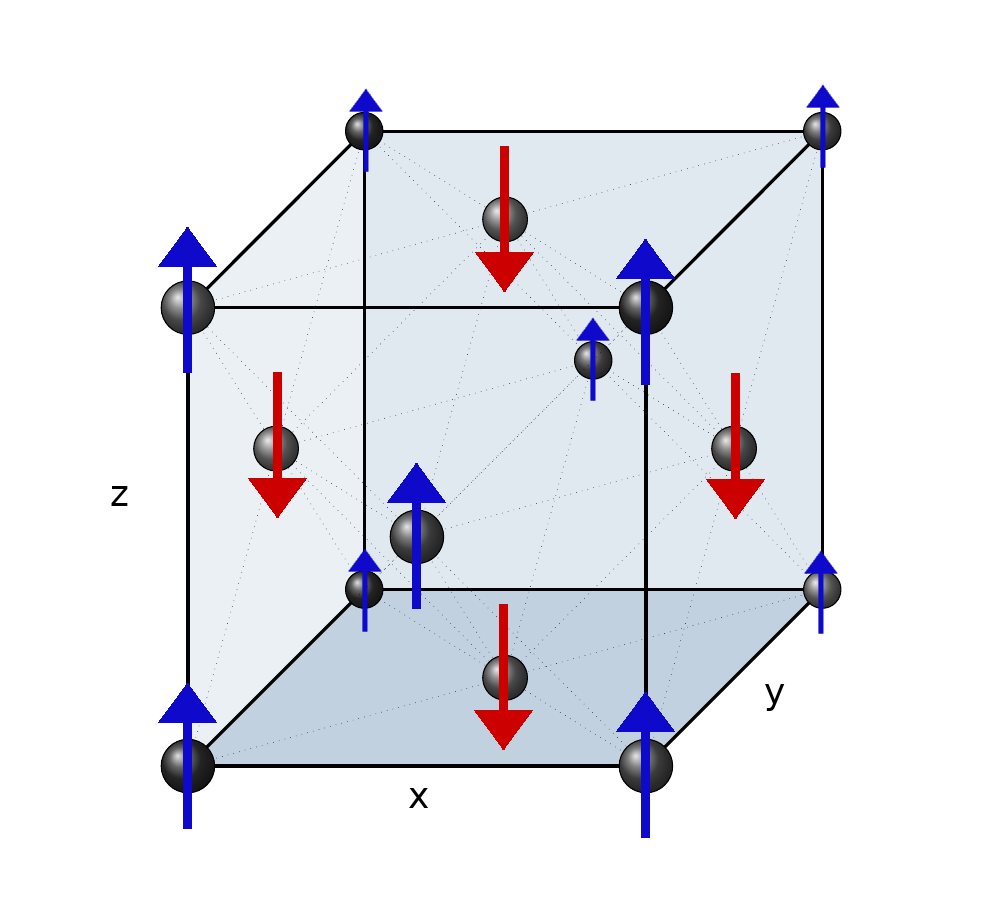
\includegraphics[width=.9\linewidth]{chapters/potentials_fe_pd_ru/images/fe-austenitic-mag.png} 
    \caption{Magnetic alignment along the z-axis, antiferromagnetic Fe fcc}  
  \end{minipage}
  \label{fig:ironfccantiferromagnetic}
\end{figure}

The atoms in the (0,1,0) plane are majority spin-up electrons, along the z-axis, and those in the (0,2,0) plane are spin-down, along the z-axis (fig. \ref{fig:ironfccantiferromagnetic}).  Following the relaxation calculation, all the atoms were in their standard \acrshort{fcc} positions, and the magnetic moment for each atom was 1.4901 \gls{bohrmagneton} and -1.4901 \gls{bohrmagneton} for the spin up and down respectively.  





%% 13.6056980659

%%%%%%%%%%%%%%%%%%%%%%%%%%%%%%%%%%%%%%%%%%%%%%%%%%%%%%%%%%%%%%%%%%%%%%%%%%%%%%%%%%%%%%%%%%%%%%%%%%%%%%%%%%
%%
%%  QEEOS
%%  
%%%%%%%%%%%%%%%%%%%%%%%%%%%%%%%%%%%%%%%%%%%%%%%%%%%%%%%%%%%%%%%%%%%%%%%%%%%%%%%%%%%%%%%%%%%%%%%%%%%%%%%%%%


\FloatBarrier
\section{QEEOS Python Code}
\label{code:qeeos}

\FloatBarrier
\subsection{Purpose of Code}

A code was developed to automate the process of calculating the equation of state and elastic constants of a material using Quantum Espresso.  It requires an input file and a starting PWscf input file.  

\begin{itemize}
\item the input configuration is relaxed using the vc-relax option in PWscf
\item configuration files are created to compute the equation of state, and PWscf is used to calculate the energies of these configurations
\item to compute the elastic constants, nine distortions are applied to the relaxed configuration with the required number of steps for each strain applied to each distortion, and these are processed with PWscf
\item once all \acrshort{dft} work has completed, the Birch-Murnaghan equation of state is fit to the first set of energies, and the nine orthorhombic elastic constants are fit to the results of the second set of energies
\end{itemize}


\FloatBarrier
\subsection{Source Code and Instructions}

The source code and instructions on how to use the program are available to download from GitHub.

https://github.com/BenPalmer1983/qe\_eos




%%%%%%%%%%%%%%%%%%%%%%%%%%%%%%%%%%%%%%%%%%%%%%%%%%%%%%%%%%%%%%%%%%%%%%%%%%%%%%%%%%%%%%%%%%%%%%%%%%%%%%%%%%
%%
%%  ELASTIC PROPERTIES
%%  
%%%%%%%%%%%%%%%%%%%%%%%%%%%%%%%%%%%%%%%%%%%%%%%%%%%%%%%%%%%%%%%%%%%%%%%%%%%%%%%%%%%%%%%%%%%%%%%%%%%%%%%%%%

\FloatBarrier
\section{Calculated Elastic Properties}
\label{section:resultselastic}

The planewave cutoff and k-points were converged to within the required parameters for energy and force but it is known that, in general, \acrshort{lda} and \acrshort{gga} pseudopotentials under and over estimate the lattice parameters.  The bulk modulus and elastic constants were calculated for \acrshort{fcc} Aluminium and \acrshort{bcc} Iron in order to compare to experimental values.

A summary of the main data points is given here for \acrshort{fcc} Al, \acrshort{bcc} Fe, \acrshort{fcc} Pd and \acrshort{fcc} Fe, and the first three listed are compared to experimental data.  A full details of the calculated properties including plots are included in appendix \ref{chapter:dftcalculatedproperties}.

\subsection{FCC Aluminium}

The parameters used for the Al calculations were arrived at earlier using the convergence code.  The remainder of the parameters are either default settings, or were selected following trial and error (for example, reducing the mixing beta to help achieve convergence).  These settings are given in table \ref{table:alfccdftsettings}.






The results in table \ref{table:alfccexperimentaldft} show a good agreement between the experimental values for Al and the calculated values.  The lattice parameter is a particularly good fit, being within 1\% of the experimental value.  The shear modulus does not match as well, but is within 20\% of the experimental value.  The \acrshort{rss} measurement of fit between the values was $2.54 \times 10^2$.



\FloatBarrier
\subsection{BCC Iron}

The equation of state and elastic constants were calculated for \acrshort{bcc} Fe, with no-spin and collinear spin.  The settings used for the calculations are given in table \ref{table:febccdftsettings}. 


The non-magnetic Iron calculation was particularly poor.  Although the lattice parameter was within 5\% of the experimental value, the structure was unstable and had negative values for both the Young's modulus and shear modulus (table \ref{table:febccexperimentaldft}).  The \acrshort{rss} measurement of fit between the values for the was $2.01 \times 10^5$.

With collinear spin enabled, the structure is stable.  The lattice parameter is still slightly under the experimental, but is now within almost 2\% of the value.  The bulk modulus predicted by fitting the Birch-Murnaghan equation of state is more than 40\% the experimental value, but the Reuss and Voigt values derived from the calculated elastic constants are just 20\% difference to the experimental value.  The latter two values are calculated using the elastic constants, rather than the equation of state.  This highlights the importance of using collinear spin calculations, despite the cost in computing time.  The \acrshort{rss} measurement of fit between the values was $1.09 \times 10^4$ giving an improvement of at least one magnitude.




\FloatBarrier
\subsection{FCC Iron}
\label{section:fccferesults}

The gamma phase of pure iron does not exist for experimental measurements to be made, and the results here will be used to fit the FCC iron potential in chapter \ref{chap:resultsfitting}.  The settings used for the calculations are given in table \ref{table:fefccdftsettings}. 

The structure is stable under the orthorhombic stability conditions given in section \ref{section:stabilityconditions}.  Whilst there are no experimental measurements to check against, the values are sane when compared to the other calculations performed here (table \ref{table:fefccexperimentaldft}).  The $C_{44}$, $C_{55}$ and $C_{66}$ values are slightly large when compared with those for \acrshort{bcc}, but further \acrshort{dft} calculations would need to be performed to investigate this.  

\begin{table}[ht]
\renewcommand{\arraystretch}{1.2}
\begin{tabular}{lccc}
\hline\hline
Property & \multicolumn{3}{c}{Value used in potential fitting} \\
\hline\hline
Element & \multicolumn{3}{c}{Fe}\\
Structure             & \multicolumn{3}{c}{Face Centered Cubic}\\
$a_0$                 & \multicolumn{3}{c}{3.59 Angstrom}\\
Nearest Neighbour     & \multicolumn{3}{c}{1.85 Angstrom}\\
Basis vectors         & $\begin{bmatrix} 0.96 & 0.0 & 0.0 \\ 0.0 & 1.00 & 0.0 \\ 0.0 & 0.0 & 0.96  \end{bmatrix}$ \\
$E_{coh}$             & \multicolumn{3}{c}{-4.32 eV}   \\
$B_0$ (GPA)           & \multicolumn{3}{c}{226.1}   \\
$E$ (GPA)             & \multicolumn{3}{c}{356.8}   \\
$G$ (GPA)             & \multicolumn{3}{c}{144.8}   \\
Poisson Ratio $\eta$  & \multicolumn{3}{c}{0.23}   \\
Elastic Constants     & $\begin{bmatrix} 364.6 & 141.6 & 233.8 & 0 & 0 & 0 \\ 141.6 & 298.7 & 130.4 & 0 & 0 & 0 \\ 233.8 & 130.4 & 364.6 & 0 & 0 & 0 \\ 0 & 0 & 0 & 186.3 & 0 & 0 \\ 0 & 0 & 0 & 0 & 266.8 & 0 \\ 0 & 0 & 0 & 0 & 0 & 186.3 \end{bmatrix}$ \\
\hline\hline
\end{tabular}
\caption{Fe input parameters for fitting}
\label{table:feinputparameters}
\end{table}








\FloatBarrier
\subsection{FCC Palladium}

The equation of state and elastic constants were calculated for \acrshort{fcc} Pd with no-spin.  The settings used for the calculations are given in table \ref{table:pdfccdftsettings}. 

There is a good agreement between the computed and experimental values for Pd, without the need to move from non-spin to collinear spin calculations (table \ref{table:pdexperimentaldft}).  However, in the alloy calculations the  presence of Fe will dictate the necessity for collinear spin.  The \acrshort{rss} measurement of fit between the values was $4.12 \times 10^3$.

\begin{table}[ht]
\renewcommand{\arraystretch}{1.2}
\begin{tabular}{lccc}
\hline\hline
Property & \multicolumn{3}{c}{Value used in potential fitting} \\
\hline\hline
Element & \multicolumn{3}{c}{PD}\\
Structure             & \multicolumn{3}{c}{Face Centered Cubic}\\
$a_0$                 & \multicolumn{3}{c}{3.925 Angstrom \cite{webelementspd}}\\
Nearest Neighbour     & \multicolumn{3}{c}{ Angstrom \cite{webelementspd}}\\
Basis vectors         & $\begin{bmatrix} 1.0 & 0.0 & 0.0 \\ 0.0 & 1.0 & 0.0 \\ 0.0 & 0.0 & 1.0  \end{bmatrix}$ \\
$E_{coh}$             & \multicolumn{3}{c}{3.91 eV \cite{semiempiricalpots}}   \\
$B_0$                 & \multicolumn{3}{c}{184.4 GPA \cite{semiempiricalpots}}   \\
Elastic Constants     & $\begin{bmatrix} 218.5 & 151.4 & 151.4 & 0 & 0 & 0 \\ 151.4 & 218.5 & 151.4 & 0 & 0 & 0 \\ 151.4 & 151.4 & 218.5 & 0 & 0 & 0 \\ 0 & 0 & 0 & 80.3 & 0 & 0 \\ 0 & 0 & 0 & 0 & 80.3 & 0 \\ 0 & 0 & 0 & 0 & 0 & 80.3 \end{bmatrix}$ \\
\hline\hline
\end{tabular}
\caption{Pd input parameters for fitting}
\label{table:pdinputparameters}
\end{table}





\FloatBarrier
\subsection{FCC Ruthenium}
\label{section:fccferesults}


Ruthenium at standard conditions exists as \acrlong{hcp}, but as this work is focused on \acrshort{fcc} steel doped with \acrshort{pgm}s, the properties are computed for \acrshort{fcc} Ruthenium.  The settings used for the calculations are given in table \ref{table:rufccdftsettings}. 



\begin{table}[ht]
\renewcommand{\arraystretch}{1.2}
\begin{tabular}{lccc}
\hline\hline
Property & \multicolumn{3}{c}{Value used in potential fitting} \\
\hline\hline
Element & \multicolumn{3}{c}{RU}\\
Structure             & \multicolumn{3}{c}{Face Centered Cubic}\\
$a_0$                 & \multicolumn{3}{c}{3.809 Angstrom \cite{webelementspd}}\\
Nearest Neighbour     & \multicolumn{3}{c}{ Angstrom \cite{webelementspd}}\\
Basis vectors         & $\begin{bmatrix} 1.0 & 0.0 & 0.0 \\ 0.0 & 1.0 & 0.0 \\ 0.0 & 0.0 & 1.0  \end{bmatrix}$ \\
$E_{coh}$             & \multicolumn{3}{c}{6.624 eV \cite{semiempiricalpots}}   \\
$B_0$                 & \multicolumn{3}{c}{307.8 GPA \cite{semiempiricalpots}}   \\
Elastic Constants     & $\begin{bmatrix} 471.5 & 219.1 & 219.1 & 0 & 0 & 0 \\ 219.1 & 471.5 & 219.1 & 0 & 0 & 0 \\ 219.1 & 219.1 & 471.5 & 0 & 0 & 0 \\ 0 & 0 & 0 & 245.0 & 0 & 0 \\ 0 & 0 & 0 & 0 & 245.0 & 0 \\ 0 & 0 & 0 & 0 & 0 & 245.0 \end{bmatrix}$ \\
\hline\hline
\end{tabular}
\caption{Pd input parameters for fitting}
\label{table:ruinputparameters}
\end{table}






%%%%%%%%%%%%%%%%%%%%%%%%%%%%%%%%%%%%%%%%%%%%%%%%%%%%%%%%%%%%%%%%%%%%%%%%%%%%%%%%%%%%%%%%%%%%%%%%%%%%%%%%%%
%%
%%  Results DFT Database
%%  
%%%%%%%%%%%%%%%%%%%%%%%%%%%%%%%%%%%%%%%%%%%%%%%%%%%%%%%%%%%%%%%%%%%%%%%%%%%%%%%%%%%%%%%%%%%%%%%%%%%%%%%%%%




\FloatBarrier
\section{DFT Configuration Database}
\label{section:dftconfigurationdbresults}


\subsection{Calibrating the Cohesive Energies}

The isolated and relaxed energy values were computed and from these values the cohesive energies were calculated (figure \ref{fig:isolatedatoms} and table \ref{table:calculatedcohesiveenergies}).  In doing so, it became apparent that there were errors of up to 12\% between the known values and those computed with \acrshort{dft}.

\begin{figure}[h]
\begin{center}
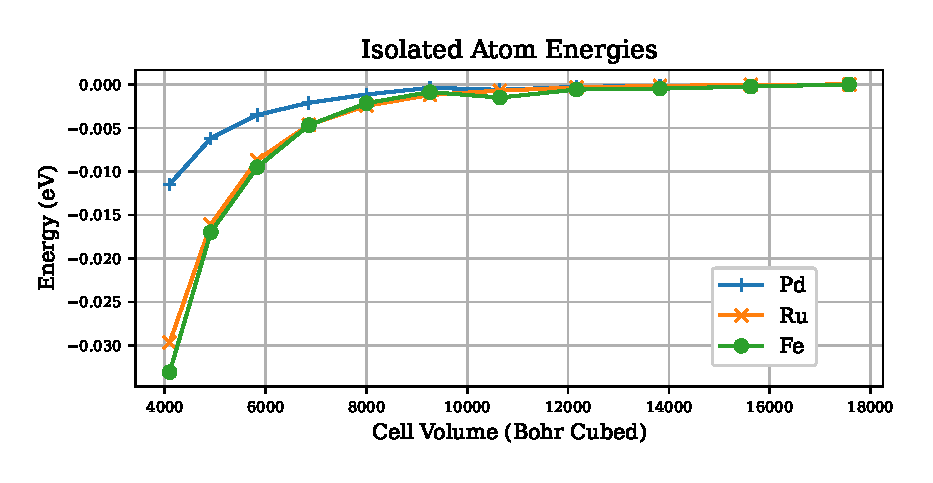
\includegraphics[width=0.5\linewidth]{chapters/potentials_fe_pd_ru/isolated/isolated_63.eps}
\caption{Isolated atom energies as cell size increase}
\label{fig:isolatedatoms}
\end{center}
\end{figure}

An offset was needed to convert from the \acrshort{dft} energies to \enquote{real} energies that could be used to derive a potential.

\begin{table}[h]
\begin{center}
\begin{tabular}{c c c c c}
\hline\hline
Element & Structure & Isolated Energy (Ry) & Relaxed Energy (Ry) & Cohesive Energy (eV) \\
\hline\hline
Fe      & BCC       & -4474.99115          & -4479.83524         & 4.84 (exp. 4.32)\\
Fe      & FCC       & -4474.99115          & -4479.78095         & 4.79 \\
Pd      & FCC       & -6962.47261          & -6966.52234         & 4.05 (exp. 3.91)\\
Ru      & HCP       & -5866.39894          & -5873.22666         & 6.83 (exp. 6.74)\\
Ru      & FCC       & -5866.39894          & -5873.11029         & 6.71 \\
\hline\hline
\end{tabular}
\end{center}
\caption{\acrshort{dft} calculated energies per atom}
\label{table:calculatedcohesiveenergies}
\end{table}

Two offsets were computed and these depend upon the settings used in the calculation (table \ref{table:calculatedoffset}).  Specifically, they depend on whether 9x9x9 k-points are used, in the case of the 32 atom calculations, or the gamma point is used (128, 129 and 256 atoms).

\begin{table}[h]
\begin{center}
\begin{tabular}{c c c c c}
\hline\hline
Element & Reference Structure & Energy (Ry) (9x9x9) & Energy (Ry) (Gamma) & Cohesive (eV)\\
\hline\hline
Fe      & BCC  & -329.2618197  & -84290.00709480 & -4.316 \\
Pd      & FCC  & -512.0299524  & -131079.09207327 & -3.91 \\
Ru      & HCP  & -431.6742014  & -110507.45936537 & -6.74 \\
\hline\hline
\end{tabular}
\end{center}
\caption{Relaxed energies for 32 atoms, using 9x9x9 k-points, and 256 atoms, using the gamma point.  These were used with the known cohesive energy to compute the offset energy.}
\label{table:calculatedoffset}
\end{table}



\subsection{Complete DFT Reference Database}

The complete database of configurations was compiled from many of the already mentioned calculations.  The QEEOS code that computed the bulk properties creates PWscf input files and processes the output files.  These output files are saved but the program and are as valid to use in the reference database as any.  In total the database has over 600 configurations for Fe-Pd and almost 600 for Fe-Ru.  

\begin{figure}
\begin{subfigure}{.32\textwidth}
  \centering
  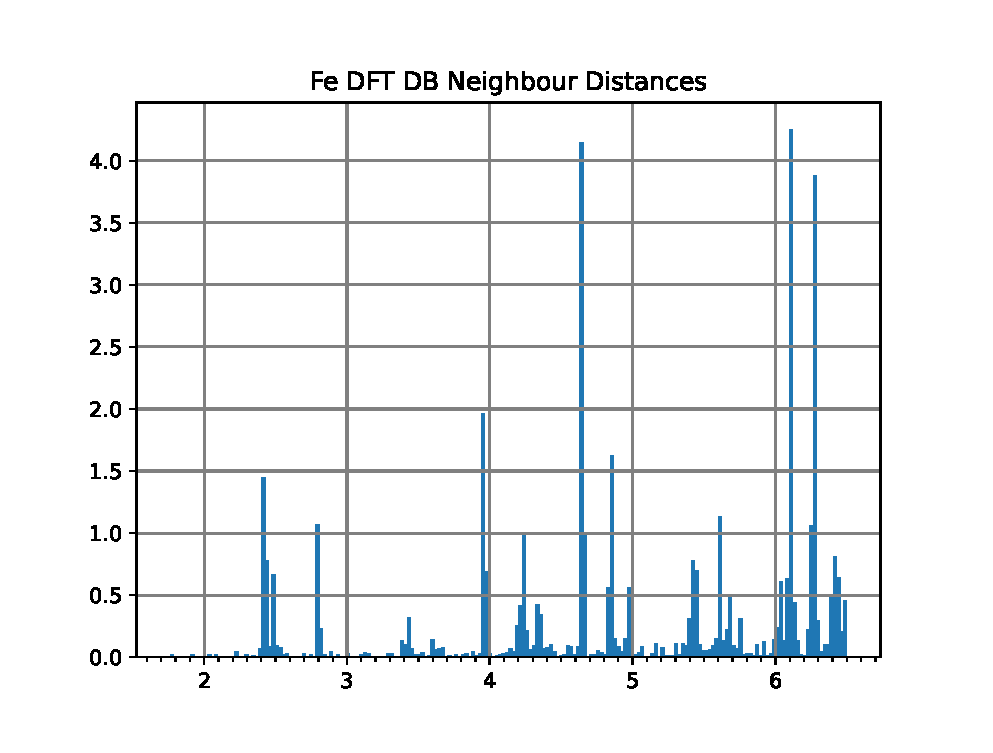
\includegraphics[width=.94\linewidth]{chapters/potentials_fe_pd_ru/neighbour_distances/db_fe_neighbours.eps}  
  \caption{Single atom, 256 atoms in total}
  \label{fig:sub-first}
\end{subfigure}
\begin{subfigure}{.32\textwidth}
  \centering
  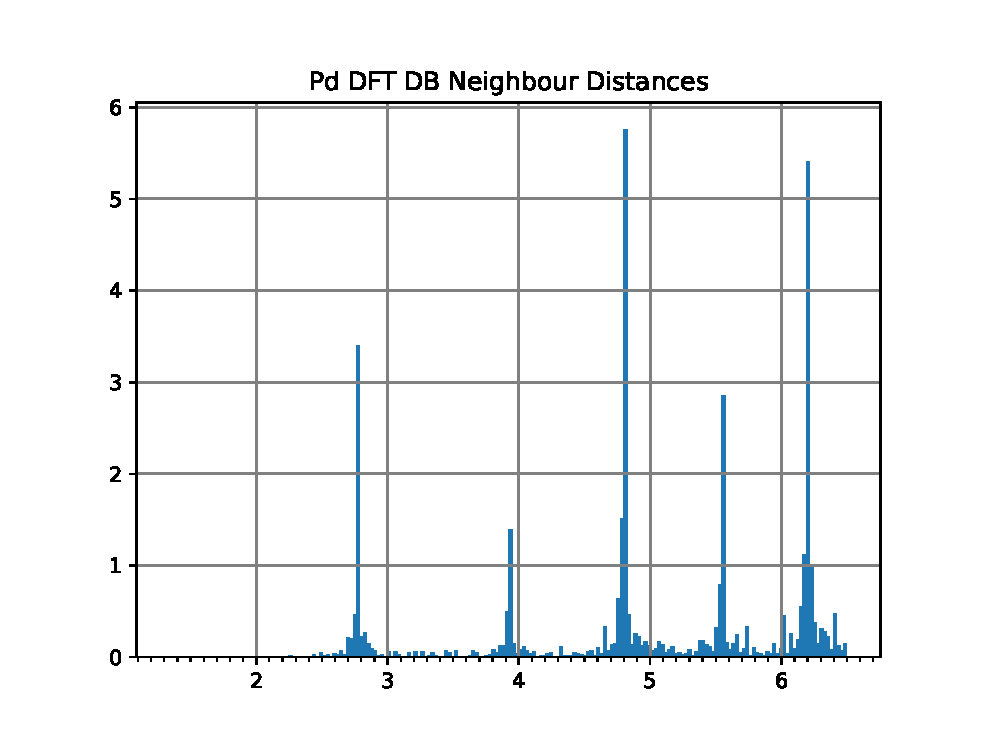
\includegraphics[width=.94\linewidth]{chapters/potentials_fe_pd_ru/neighbour_distances/db_pd_neighbours.eps}  
  \caption{Multiple atoms, 256 atoms in total}
  \label{fig:sub-first}
\end{subfigure}
\begin{subfigure}{.32\textwidth}
  \centering
  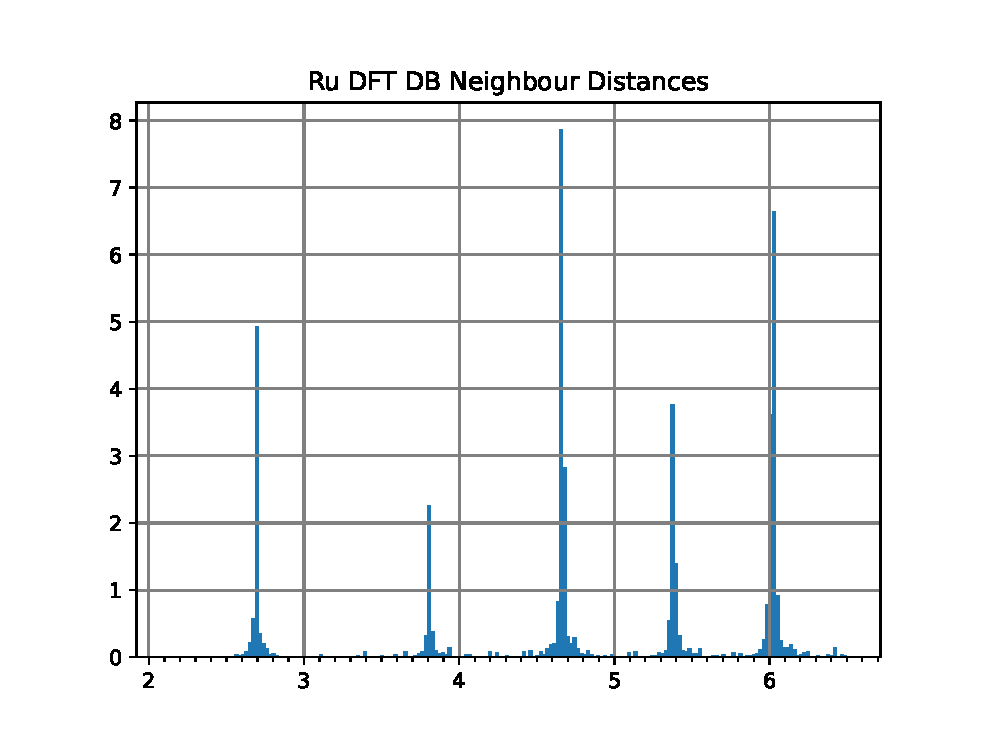
\includegraphics[width=.94\linewidth]{chapters/potentials_fe_pd_ru/neighbour_distances/db_ru_neighbours.eps}  
  \caption{Multiple atoms, 256 atoms in total}
  \label{fig:sub-first}
\end{subfigure}
\begin{subfigure}{.32\textwidth}
  \centering
  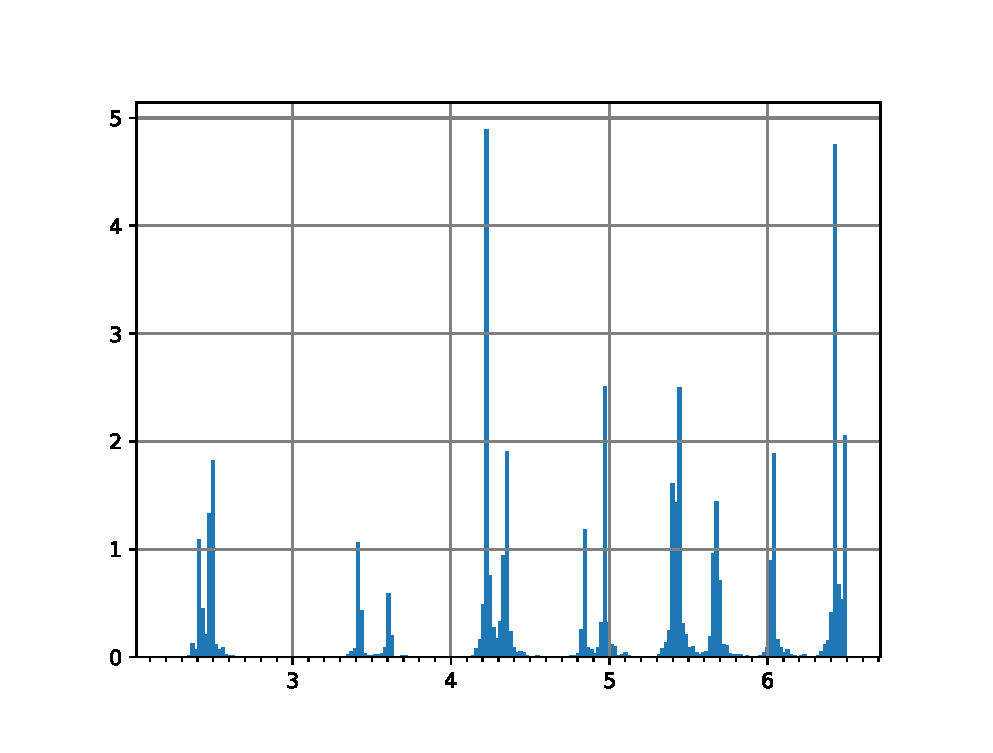
\includegraphics[width=.94\linewidth]{chapters/potentials_fe_pd_ru/neighbour_distances/db_fepd_neighbours.eps}  
  \caption{Multiple atoms, 256 atoms in total}
  \label{fig:sub-first}
\end{subfigure}
\begin{subfigure}{.32\textwidth}
  \centering
  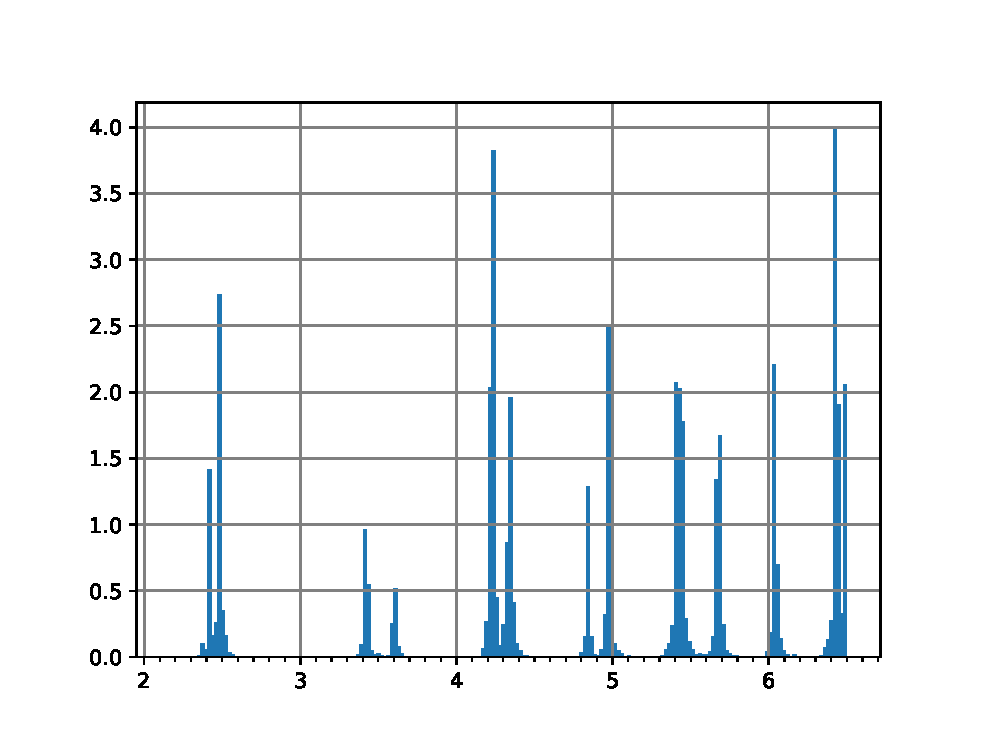
\includegraphics[width=.94\linewidth]{chapters/potentials_fe_pd_ru/neighbour_distances/db_feru_neighbours.eps}  
  \caption{Multiple atoms, 256 atoms in total}
  \label{fig:sub-first}
\end{subfigure}
\label{fig:dbneighbourseparations}
\end{figure}

The distribution of atom separations was measured across the database and these are plotted in figure \ref{fig:dbneighbourseparations}.  The full set is available to download from https://github.com/BenPalmer1983/fepd\_feru\_potential.


















%%%%%%%%%%%%%%%%%%%%%%%%%%%%%%%%%%%%%%%%%%%%%%%%%%%%%%%%%%%%%%%%%%%%%%%%%%%%%%%%%%%%%%%%%%%%%%%%%%%%%%%%%%
%%
%%  EAMPA Code
%%  
%%%%%%%%%%%%%%%%%%%%%%%%%%%%%%%%%%%%%%%%%%%%%%%%%%%%%%%%%%%%%%%%%%%%%%%%%%%%%%%%%%%%%%%%%%%%%%%%%%%%%%%%%%

\FloatBarrier
\section{EAMPA Python Code}
\label{code:eampa}


%%%%%%%%%%%%%%%%%%%%%%%%%%%%
% Introduction
%%%%%%%%%%%%%%%%%%%%%%%%%%%%

\subsection{Introduction}

This code was developed to analyse interatomic potentials and fit their parameters to data.  It currently has the following features:

\begin{itemize}
\item calculate energy, forces and stress of an ensemble of atoms 
\item calculate bulk properties of a potential for pure \acrshort{bcc} of \acrshort{fcc} structures
\item fit parameters using simulated annealing, genetic algorithm, Nealder-Meade, Levenberg-Marquardt, BFGS
\item  
\end{itemize}

The source code and instructions on how to use the program are available to download from GitHub.

https://github.com/BenPalmer1983/eampa

After several iterations, a Python-Fortran version was developed.  The Python code was designed to handle the user input, output and the fitting process.  The Fortran modules were designed with a separate module for each task: energy/force/stress, bulk properties, surface energy and defect calculations.  The surface energy and defect module is incomplete.  More modules may be easily added at a later date.



%%%%%%%%%%%%%%%%%%%%%%%%%%%%
% Potentials
%%%%%%%%%%%%%%%%%%%%%%%%%%%%

\subsection{Potentials}

The code has been designed specifically for many body potentials.  These include \acrlong{fs},  \acrlong{eam}, \acrlong{2beam} but not the \acrlong{meam}.  It may be reduced to pair potentials only by setting the density function and embedding functional to \enquote{zero} (see appendix \ref{chapter:potentialfunctions} for function details).  

The function types available for pair, density and embedding are listed in the appendix (\ref{chapter:potentialfunctions}).  More function types may be easily added by editing the Fortran fnc module and recompiling the efs and bp modules.

Most of the functions are basic mathematical functions that use built in operators and functions.  Several are more complex, such as the cubic spline, quintic spline and knot-to-knot splines.


\subsubsection{Cubic and Quintic Splines}

These splines have been discussed in section \ref{section:backgroundpolynomialsplines}.  Several papers have previously used summed polynomial splines that employ the Heaviside-step function to cut off these functions at the desired points.  The cubic term, $(r - r_i)^3$, ensures the function and it's first and second derivatives equal zero and are continuous at the cutoff points.  

\begin{equation}
\begin{split}
V(r) = \sum_i^N a_i (r - r_i)^3 H(r_i - r) \\
\text{where } \\
H(x) = \left\{ \begin{matrix} 0 & x<0 \\  1 & x >= 0 \end{matrix} \right . 
\end{split}
\label{eq:cubicSpline}
\end{equation}

This was implemented in Fortran so that an efficient vectorised version could be used by Python.  The Fortran code for the spline function is in the appendix \ref{section:appendixcubicspline}.


\subsubsection{Knot to Knot Splines}

A Fortran module was created for the knot-to-knot spline function.  It takes a set of knots and splines between the knots pair at a time using the x, y, y' values to construct a set of linear equations to solve. 

\begin{equation}
  \begin{split}
    c_0 + c_1 x_A + c_2 {x_A}^2 + c_3 {x_A}^3 = f(x_A) \\
    0 + c_1 + 2 c_2 {x_A} + 3 c_3 {x_A}^2 = f'(x_A) \\
    c_0 + c_1 x_B + c_2 {x_B}^2 + c_3 {x_B}^3 = f(x_B) \\
    0 + c_1 + 2 c_2 {x_B} + 3 c_3 {x_B}^2 = f'(x_B) 
  \end{split}
  \label{eq:eqSplineThreeEquations}
\end{equation}


\begin{equation}
  \begin{split}
    \begin{bmatrix}
    1  &  x_A  &  {x_A}^2  &  {x_A}^3     \\
    0  &  1    &  2 x_A    &  3 {x_A}^2   \\
    1  &  x_B  &  {x_B}^2  &  {x_B}^3     \\
    0  &  1    &  2 x_B    &  3 {x_B}^2
    \end{bmatrix}
    \begin{bmatrix}
    c_0 \\
    c_1 \\ 
    c_2 \\ 
    c_3
    \end{bmatrix}
    = 
    \begin{bmatrix}
    f(x_A) \\
    f'(x_A) \\ 
    f(x_B) \\ 
    f'(x_B)
    \end{bmatrix}
  \end{split}
  \label{eq:eqSplineThreeMatrix}
\end{equation}


A subroutine was created to calculate the coefficients for the 3rd order or 5th order polynomial to spline the two knots.  This subroutine and the remainder of the module are available to view and download on the GitHub repository for this project.  The Fortran code for a cubic and cubic with \acrshort{zbl} inner core knot-to-knot spline are included in the appendix (section \ref{section:appendixcubicknotspline} and section \ref{section:appendixcubicknotsplinezbl}).





%%%%%%%%%%%%%%%%%%%%%%%%%%%%
% Calculations
%%%%%%%%%%%%%%%%%%%%%%%%%%%%



\subsection{Calculations}

The calculations involved in this code centre around the calculation of energy of configurations as well as the forces and stresses when necessary.  All configurations are held within the Python program, but the neighbour list and energy (as well as stress and force) calculations are carried out in an imported Fortran module.

\subsubsection{Energy, Force and Stress Calculations}

A potential and configuration of atoms may be loaded into the program in a number of ways.  Python passes this data to the atom Fortran module.  This computes the neighbour list and this is passed back to the Python program where it is stored for later use.

There are a number of functions that allow the potential as well as atom configurations (and neighbour lists) to be updated.  These are handled in Python, but the calculations are carried out in the Fortran atom module, that then passes the results back to Python.

The energy, forces and stresses may be computed for a range of configurations or a single configuration.  This process starts in Python, but the heavy lifting is once again completed using the Fortran module.  The method used is discussed in section \ref{section:backgroundenergyforcestress} and the subroutine used is included in the appendix (section \ref{section:appendixenergyforcestress}).


\subsubsection{Geometry and Coordinate Optimisation}

Once a configuration is loaded into the program, it can be relaxed using a variety of techniques.  The lattice parameter may be relaxed using the built in \acrshort{bfgs} or \acrshort{cg} minimizers.  The same functions may be used to relax the simulation cell.  Where the coordinates of the atoms are relaxed, a damped molecular dynamics subroutine is called from the Fortran module that computes the forces on the atoms and moves them accordingly.  This has been more successful than using built in minimizers, where no gradient data is passed, but a more promising approach might be to include the VA08 subroutine from the Harwell archives\cite{harwellva08}.  This is the same subroutine used in the Bonny potential fitting code\cite{bonnyfecr}.



\subsubsection{Bulk Property Calculations}

The bulk property calculations rely on the calculation of energy of a number of configurations where specific strains


The bulk property calculations are also performed in Python using a library created with F2PY.  In order to speed up the calculation, the equation of state and elastic constant configurations use the known lattice parameter set by the user.  The methods used are discussed in chapter \ref{chap:backgroundfitting} and the subroutine that creates the configurations, with which the module calculates the energies used to plot the equation of state and other distortions, is included in the appendix \ref{section:appendixbpaddconfiguration}.


\subsubsection{RSS - How Well The Potential Fits Experimental \& DFT Data}

The fitting process measures how well a potential fits the data when the initial parameters are given and every time a new set of parameters are proposed.  They are weighted and computed in the efs and bp modules.  They are the \acrfull{rss} of the differences between calculated energies, forces, stress, lattice parameter, cohesive energy, bulk modulus and elastic constants and the known values.  The sum of these values measures how well the potential fits.


\subsection{Analytic Potential Fitting}

In earlier versions, the code used tabulated potentials only.  Any analytic potentials were converted to tabulated.  This was for two reasons: the functions could be easily exported and used by other codes that may not have the same analytic functions, and interpolation between tabulated data was faster to compute the value and gradient of a function at a certain point than several of the analytic functions (in particular the knot-to-knot splines).  

A negative aspect is that, whilst the pair and density functions have a fixed range (from 0 to the cutoff radius), the range for the embedding functional depends on the density function, and the range of densities computed at each atom location.  Rather than compute this first, I re-wrote the code to use analytic functions only, with the option of outputting as a tabulated function for use in other programs.  A number of Python scripts were created to fit pre-existing tabulated potential functions into analytic functions to use as a starting point for the fitting procedure.

\subsection{Overview of the Potential Fitting Process}

The input files are read in by Python that then iterates over the fitting process while changing the potential.  The Fortran modules calculate the energy, force and stress of the loaded configurations as well as the bulk property calculations for pure crystals of the atomic species and structures specified by the user.  To save on processing time, the neighbour lists for all configurations, including those used to calculate the equation of state and elastic constants, are only calculated once. 

The step by step flow of the program while fitting parameters of a potential is as follows:

\begin{enumerate}
\item Read input files
\item Load Fortran Modules
\item Load potentials into Python and Fortran
\item Load configurations into Python and Fortran
\item Allocate memory
\item Create neighbour list for all configurations
\item Create eos and ec configurations and neighbour lists
\item Begin fitting loop in Python
\item Loop starts - loop through potential function parameters
\begin{enumerate}
\item Update potential and load parameters to Fortran modules
\item Loop starts - loop through configurations
\begin{enumerate}
\item Calculate energy, force, stress using pre-calculated neighbour lists
\end{enumerate}
\item End loop
\item Loop starts - bulk property calculations for each pure element
\begin{enumerate}
\item Calculate eos and ec values and bulk properties using pre-calculated neighbour lists
\end{enumerate}
\item End loop
\item Calculate rss between these values and known/dft
\item Save parameters if best
\item Make new parameters
\end{enumerate}
\item End loop
\item Output results
\end{enumerate}

Once the fitting process has completed, the best set of parameters are stored for the user along with a plot of the potential functions, equation of state and elastic constant energy-strain distortion plots (where these are used in the fitting process).





\subsection{Simulated Annealing}

The simulated annealing algorithm was considered for optimisation, and may be implemented as an option in the future.  The algorithm looks for better solutions and replaces the current value with better values.  It also accepts worse solutions with a probability that decreases with \enquote{temperature}.  Similar to the way atoms find optimal positions by annealing and cooling, the algorithm starts with a high temperature and it reduces this temperature over time.  It is used to search for the global optimum.

The algorithm used is given in the appendix (section \ref{section:simulatedannealing}).




\subsection{Genetic Algorithm}

The global optimum is searched for using a genetic algorithm.  The user chooses the parameters for the algorithm and it attempts to search for the optimum parameters to fit the potential functions to the data.

The user settings include the following:

\begin{itemize}
\item population size
\item \enquote{fresh} (new randomly generated) parameters
\item number of generations
\item number of extinction events
\item how often the top solutions are enhanced with linesearch and gradient descent
\end{itemize}

The subroutine that breeds the parameters randomly combines the parameters from two parent solutions to create two children parameter sets.  The parents are either both from the existing pool of solutions, or a parent from the existing pool with a parent from a fresh set, and the fresh set of parameters changes with each generation (fig. \ref{fig:gabreedevent}).

\begin{figure}[h]
  \begin{center}
    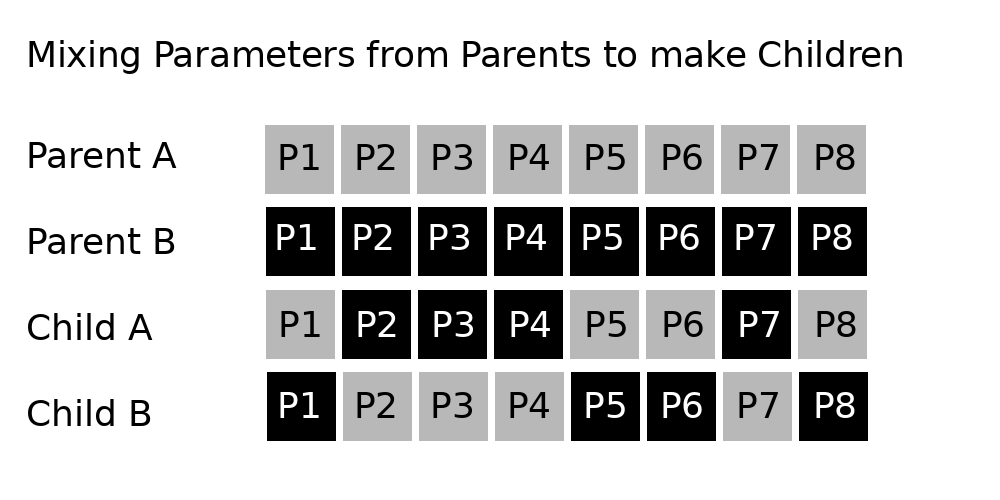
\includegraphics[scale=0.30]{chapters/potentials_fe_pd_ru/images/breeding.png}
    \caption{Parameter Breed Event}
    \label{fig:gabreedevent}
  \end{center}
\end{figure}

There is a chance that the child solutions will mutate slightly from the two parent combination, and this chance is set by the user.

During the breed event, the program will check whether or not the two children already exist within the solution pool.  If they are allowed to also enter the pool, the solutions may quickly be filled with clones during the breeding process.  The breed event automatically forces any clones to be varied so they become a different and distinct solution.

Every now and then an extinction event will occur that kills off any poor solutions and replaces them with variations of the better solutions.  The user controls the frequency of the extinction event and the probability that a solution will be removed.

Top solutions are enhanced, at a frequency picked by the user, using a local optimisation algorithm: line-search and gradient descent.  It does require many calculations and adds a substantial amount of time to the procedure, but it uses the gradient of solutions to find more optimal solutions more efficiently that randomly generated or bred solutions.

The algorithm used is given in the appendix (section \ref{section:geneticalgorithm}).


\subsection{Newton Gauss Optimisation}

The Newton Gauss optimisation estimates the second order derivatives matrix, the Hessian, by multiplying the Jacobian and its transpose.  It is not yet implemented in the code, but may be in the future.  The algorithm is used to find a local optimum, but it can be unstable or return errors.

\begin{equation}
\begin{split}
\vec{J}^{T} \vec{J} \vec{p} = \vec{J}^{T} \vec{r} \\
\vec{r} = \vec{y} - f(\vec{x}, \vec{p})
\end{split}
\label{eq:eqNewtonGauss}
\end{equation}

\subsection{Levenberg-Marquardt Optimisation}

The Levenberg-Marquardt algorithm is similar to the Newton-Gauss method, but the estimate for the Hessian does not need to be calculated for each loop of the algorithm.  The parameter, $\lambda$, is changed and the Hessian is updated periodically.  This is not yet implemented in the code, but may be added in the future.

\begin{equation}
\begin{split}
\left( \vec{J}^{T} \vec{W} \vec{J} + \lambda diag\left( \vec{J}^{T} \vec{W} \vec{J} \right) \right) \vec{p} = {\left(\vec{J}^{T} \vec{W} \vec{r} \right)} \\
\vec{r} = \vec{y} - f(\vec{x}, \vec{p})
\end{split}
\label{eq:eqLevenbergMarquardt}
\end{equation}


\subsection{Python SciPy Optimization Functions}

Additional optimisation functions have been used by importing the SciPy module into the program, and these may be used in conjunction with those listed above.  Several have been used including the bin-hopping, Nealder-Meade and \acrshort{bfgs}.  The bin-hopping was unreliable and crashed on a number of occasions, so I used the simulated annealing and genetic algorithms programmed specifically for this work.  The Nealder-Meade and \acrshort{bfgs} were both used following the run of global optimisation and increased the efficiency of improving the parameters.








\subsection{Minimising Runtime}

\subsubsection{Python, Fortran \& OpenMP}

When fitting a potential, for each trial set of functions, the program must calculate the energy, forces and stress for each of the configurations and tens or hundreds of energy only calculations for the equation of state and elastic constant calculations.  Python is a well used programming language in many areas of Science and it has the benefits of many modern languages.  For certain specific tasks, it is slow in comparison to Fortran.

The energy, stress and force calculations were programmed in Fortran and use OpenMP to calculate the many configurations in parallel.  On a single thread, the fitting process could take weeks, but on a 20 core node the calculation time was reduced to under a couple of days.

\subsubsection{Function Caching}

not relevant

The first version of the code used tabulated potentials, and this removed the task of programming different functions (and the wide range of complexities amongst those functions) and replaced it with a quick search and interpolation of tabulated data.  However, the final version was developed to use and fit with analytic potentials.  Several of the optional functions, including the knot-to-knot spline function, drastically increased the computational time.  

The bulk property module in particular uses configurations with atoms in regular places, with there being a small set of unique atom separation values.  Rather than generate tabulated data for each function, to then interpolate, the input and output values are cached.  Once the value is calculated, it is quickly retrieved for subsequent calculations with the same input value.  The has increased computation speed of the analytic potentials to a speed similar to using tabulated functions.



\subsection{Interpolation for Non Analytic Potentials}

In the current version, only analytic potentials are available for fitting.  There are several subroutines ready if tabulated functions are reintroduced.  These subroutines use Lagrange polynomials to interpolate values of the function (eq. \ref{eq:eqLagrangeDataSet} \ref{eq:eqLagrangePolynomialNew}).

\begin{equation}
\begin{split}
D = \lbrace \left(x_0, y_0 \right) \left(x_1, y_1 \right) \left(x_2, y_2 \right) \dotsm \left(x_n, y_n \right) \rbrace
\end{split}
\label{eq:eqLagrangeDataSet}
\end{equation}

\begin{equation}
\begin{split}
p_n (x) = \sum _{i=0} ^n y_i L(i, x) 
\textnormal{where    } l(i, x) = \prod _{j=0 , j!=i} ^n (x - x_j)
\end{split}
\label{eq:eqLagrangePolynomialNew}
\end{equation}

There are typically hundreds or thousands of data points, so to interpolate, the closest few points are used.  Throughout the computer code four point interpolation was the preferred method, to balance computational speed with a well fitting polynomial.  

The gradient of the potential functions are also computed using Lagrange polynomials (eq. \ref{eq:eqLagrangePolynomialNew}).

%% Sample hybrid function
\begin{equation}
\begin{split}
q_n \left( x \right) = \sum_{i=0}^{i=n} y_{i} g \left(i,  x \right) \\
\textnormal{where    } g \left(i, x \right) = \left( \prod_{j=0, j \neq i}^{j=n} \frac{1}{x_i - x_j} \right) \times \left( \sum_{k=0, k \neq i}^{k=n} \prod_{j=0, j \neq k, j \neq i}^{j=n} \left( x - x_j \right) \right)
\end{split}
\label{eq:eqLagrangePolynomialNew}
\end{equation}

A pseudocode for both interpolation of the function points and derivatives are available in the appendix (section \ref{section:interpolationpseudo} and \ref{section:interpolationgradientpseudo}).



\subsection{Effective Gauge Transforms}

In order to create a potential for an alloy an effective gauge transform, as described in section \ref{section:pairembeddingsym}, was applied to each pure potential.  A mode added to the EAMPA program reads in the analytic potential and creates a numeric potential that has had the transform applied.  This allows the pure potentials to be used together, although a cross pair potential is still needed.



%%%%%%%%%%%%%%%%%%%%%%%%%%%%%%%%%%%%%%%%%%%%%%%%%%%%%%%%%%%%%%%%%%%%%%%%%%%%%%%%%%%%%%%%%%%%%%%%%%%%%%%%%%
%%
%%  Potentials
%%  
%%%%%%%%%%%%%%%%%%%%%%%%%%%%%%%%%%%%%%%%%%%%%%%%%%%%%%%%%%%%%%%%%%%%%%%%%%%%%%%%%%%%%%%%%%%%%%%%%%%%%%%%%%



\FloatBarrier
\section{Iron-Palladium Potential}
\label{section:fepdpotentialresult}

\subsection{Reference Database}

The database of reference configurations discussed in chapter \ref{chap:resultsdftdb} was used to derive this potential.  It was designed for \acrshort{fcc} Fe rather than \acrshort{bcc} Fe, and this is one point that distinguishes this potential from those that already exist.

During the fitting process, there was a desire to have a reasonably good fit to bulk property values as well as the defect configurations, perturbed atom configurations and so on.  This was quite a challenge to fit to so many variables and as a result more weight was given to the bulk and slab/surface configurations.

There were a number of options available when choosing certain parameters, such as using \acrshort{dft} to compute cohesive energies based on relaxed and isolated configurations, or to extrapolate based on known energies.  The choices made are listed below and these apply to both the Fe-Pd and Fe-Ru potential.

\begin{itemize}
\item all cohesive energies were computed based on known experimental values and the \acrshort{dft} computed relaxed energy of those structures
\item all bulk property values are those computed using \acrshort{dft}
\end{itemize}
 

\subsection{Potential}

The full potential is available from https://github.com/BenPalmer1983/fepd\_feru\_potential and is ready to use with \acrshort{lammps}.



\begin{figure}[htb]
\begin{subfigure}{.32\textwidth}
  \centering
  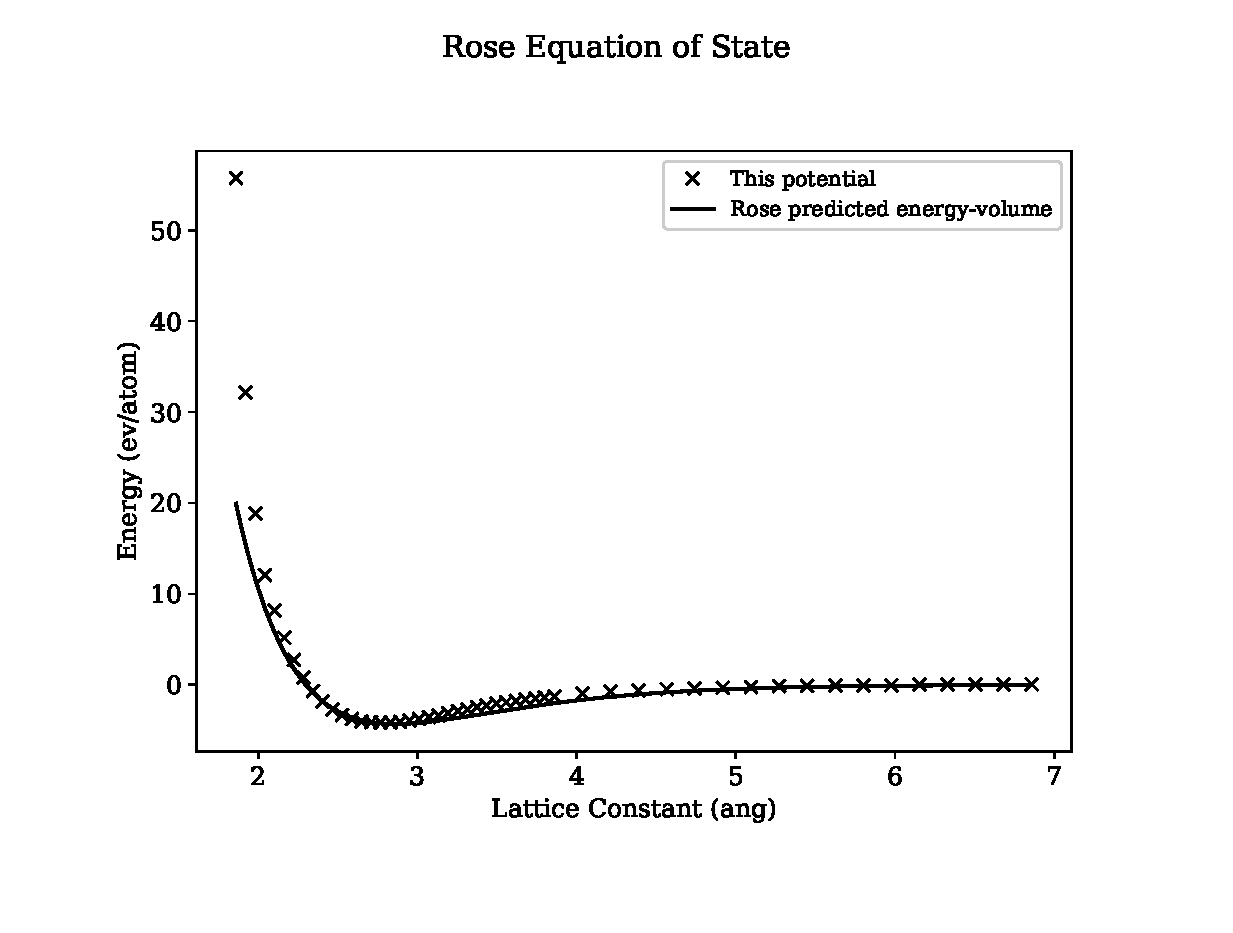
\includegraphics[width=.94\linewidth]{chapters/potentials_fe_pd_ru/fepd_potential/rose_plot_bp_0.eps}  
  \caption{BCC Iron}
  \label{fig:sub-first}
\end{subfigure}
\begin{subfigure}{.32\textwidth}
  \centering
  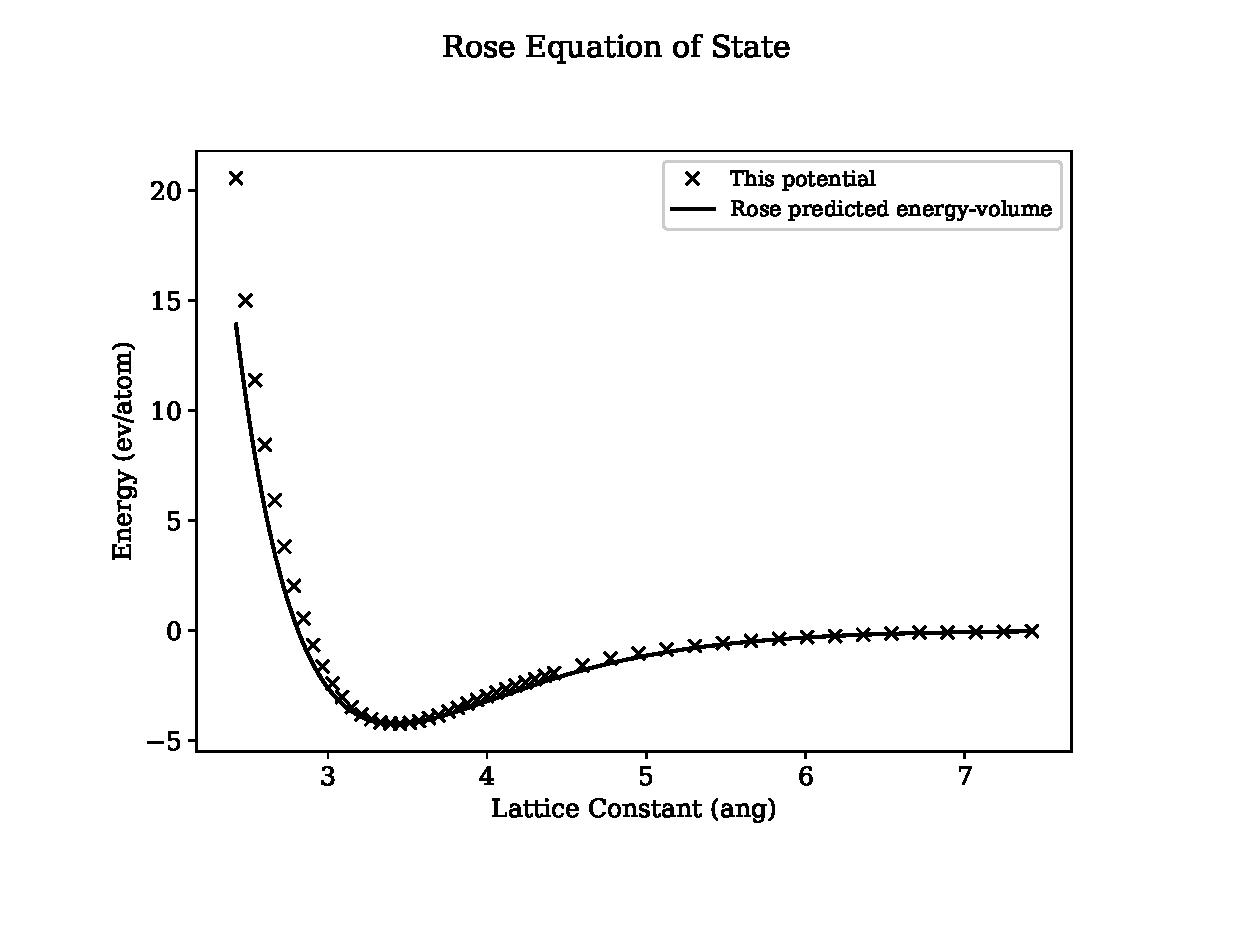
\includegraphics[width=.94\linewidth]{chapters/potentials_fe_pd_ru/fepd_potential/rose_plot_bp_1.eps}  
  \caption{FCC Iron}
  \label{fig:sub-first}
\end{subfigure}
\begin{subfigure}{.32\textwidth}
  \centering
  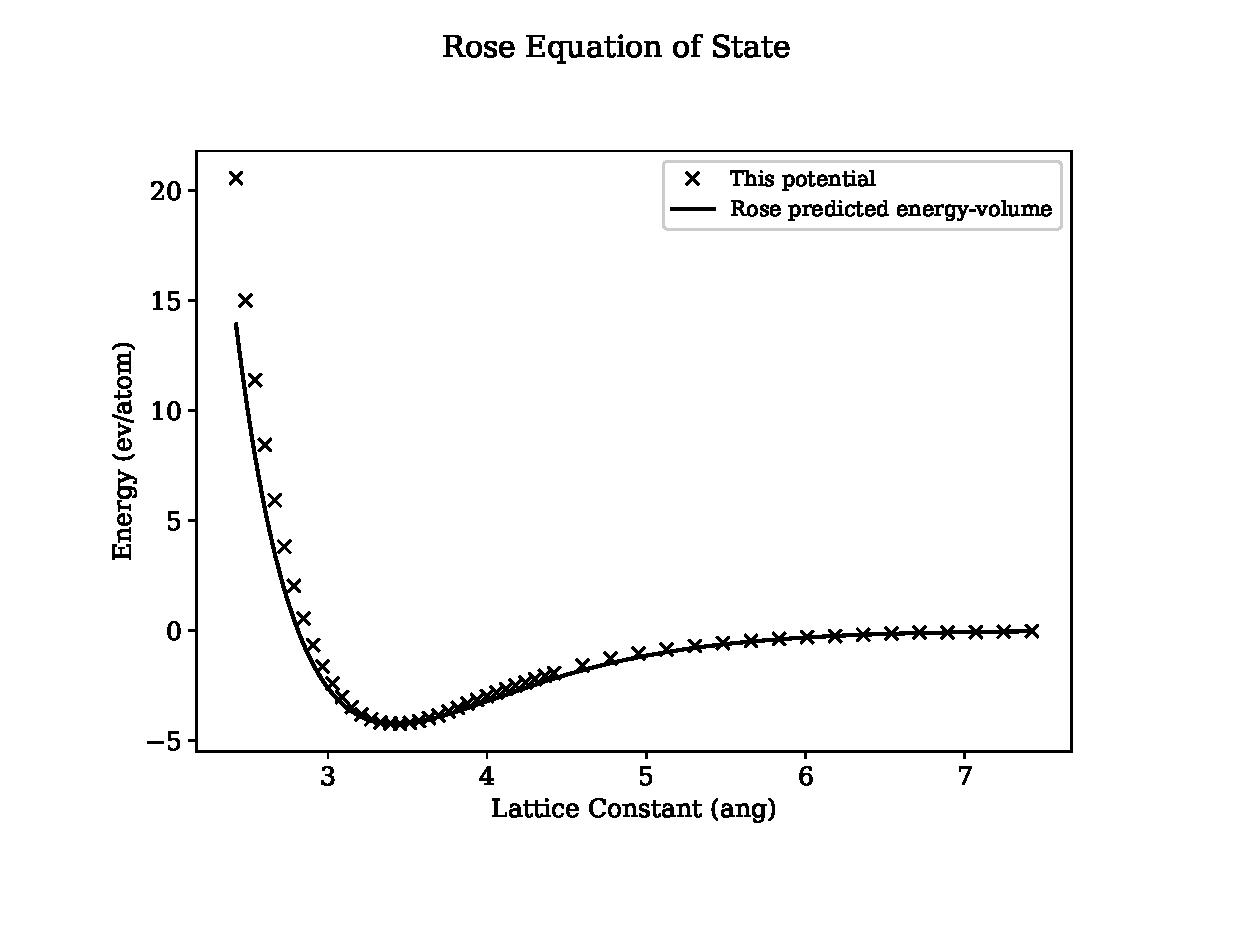
\includegraphics[width=.94\linewidth]{chapters/potentials_fe_pd_ru/fepd_potential/rose_plot_bp_1.eps}  
  \caption{FCC Palladium}
  \label{fig:sub-first}
\end{subfigure}

\label{fig:binaryalloyconfigurationsbulk}
\end{figure}





















































%%##################################################################################################
%%
%%
%%     Removed 
%%
%%
%%##################################################################################################



\begin{comment}




In order to perform \acrshort{md} ion damage simulations, an iron-palladium potential is needed.  Experimental data is available for FCC palladium, but \acrshort{dft} is needed to compute the properties of FCC iron, as it does not exists in this phase at standard conditions without the addition of an austenite stabilizer.  Additional \acrshort{dft} calculations will be used to compute the energy, stress and forces of slightly perturbed atoms which will in turn be used to fit the potentials.  A new computer code will be created to fit the potentials.\\
\\
The key parameters required for Quantum Espresso are converged and selected in preparation for the upcoming calculations.  A set of atom configurations for \acrshort{fcc} crystals are created and \acrshort{dft} is used to computer the energy, forces and stresses on these crystals.\\ 
\\ 
\acrshort{fcc} iron does not exist at normal room temperature and pressure, without the addition of a austenite stabiliser.  A set of \acrshort{dft} calculations are used to compute the bulk modulus, lattice parameter and cohesive energy of pure Fe \acrshort{fcc}.  Ruthenium has a \acrshort{hcp} structure and similarly \acrshort{dft} calculations are used to compute bulk properties of \acrshort{fcc} Ruthenium.\\
\\
The database of bulk properties and atom configuration are used in chapter \ref{chap:resultsfitting} to derive potentials for both Fe-Pd and Fe-Ru as well as for the pure elements.\\
\\
A computer code was developed to fit interatomic potentials to \acrshort{dft} calculated energy, force and stress data.  It also uses bulk property data including the bulk modulus, lattice parameter, cohesive energy and elastic constants.  It was written in Python and Fortran and has been designed to be easy to add new fitting data, such as cohesive energy and surface energy plots.
\\
The code has been used with the results from chapter \ref{chap:resultsdftdb} to fit two potentials for \acrshort{fcc} Fe-Pd.  The cohesive energy and surface energy plots were calculated using these potentials.


















\subsection{Potential Functions \& Functionals}

There are a large number of functions and functionals used in the literature, and the potentials provided by H. Sheng are numeric\cite{shengeam} (section \ref{section:shengeampotentials}).  In this work, it was decided to use a knot-to-knot spline for the pair potential that is attached to a ZBL potential for small separations, with a fixed node at the cutoff, with a zero value and gradient.  In the first instance the radial electron density was calculated using DIRAC and from this a knot-to-knot spline was fitted with a forced cutoff to $\rho(r_{cut}) = 0, \rho'(r_{cut}) = 0$.  This was then replaced with a knot-to-knot spline based on the Sheng density potentials and the reason for this will be discussed in section \ref{section:diracdensityplots}. Finally, the embedding functionals take the form $f(x) = p(1) \times \sqrt{r} + p(2) \times r^2$ as used by Mendelev\cite{femendelev}\cite{feacklandmendelev}, Ackland\cite{feacklandmendelev}, Olsson\cite{olssonfecr} and Wallenius\cite{olssonfecr}.





\FloatBarrier
\subsubsection{Sheng Potentials}

The Sheng potentials available are numeric and so the functions used in this work were first fit to the tabulated data\cite{shengeamonline}.  As the Sheng Pd is a potential for a \acrshort{fcc} crystal, this was a starting point for both Fe and Pd (which is quite obvious for the case of Pd).  Plot for the Pd potential are given in figs. \ref{fig:shengpdpair} \ref{fig:shengpdpairzoom} \ref{fig:shengpddens} \ref{fig:shengpdembe}.

\FloatBarrier
\begin{figure}[htb]
\minipage{0.49\textwidth}
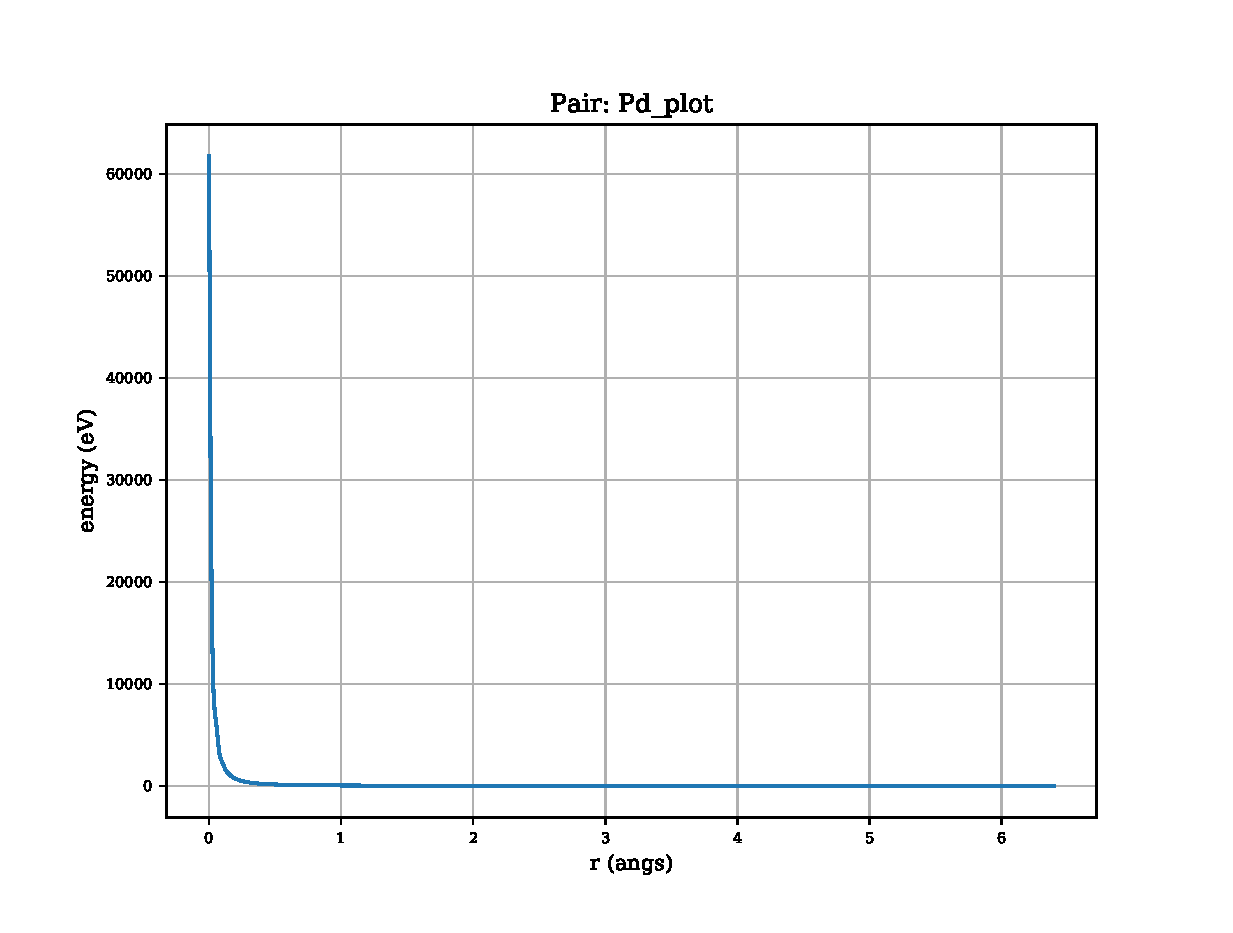
\includegraphics[width=\linewidth]{chapters/potentials_fe_pd_ru/sheng/Pd_plot_pair.eps}
\caption{Sheng palladium pair function}
\label{fig:shengpdpair}
\endminipage\hfill
\minipage{0.49\textwidth}
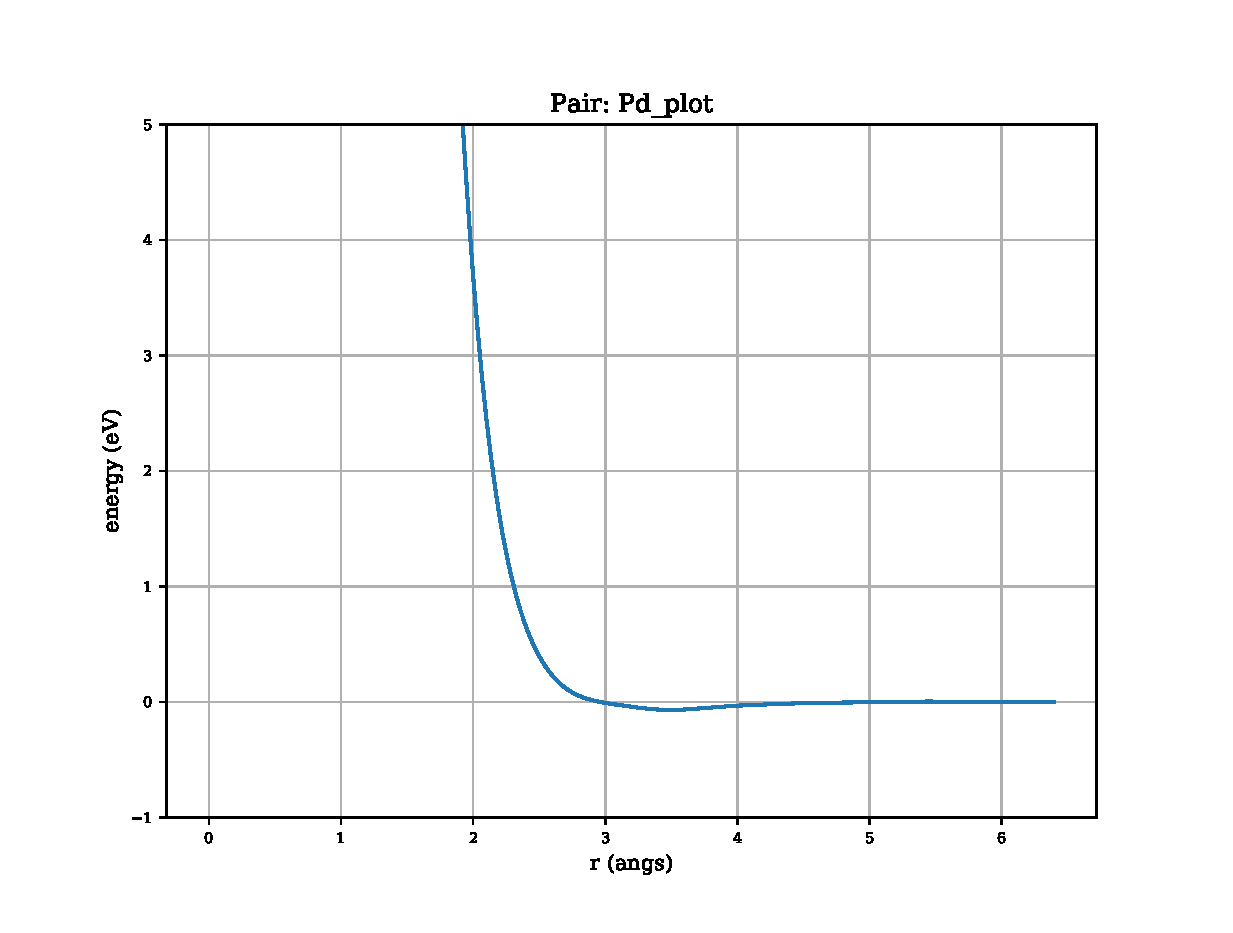
\includegraphics[width=\linewidth]{chapters/potentials_fe_pd_ru/sheng/Pd_plot_pair_zoomed_in.eps}
\caption{Sheng palladium pair function (zoomed in)}
\label{fig:shengpdpairzoom}
\endminipage

\minipage{0.49\textwidth}
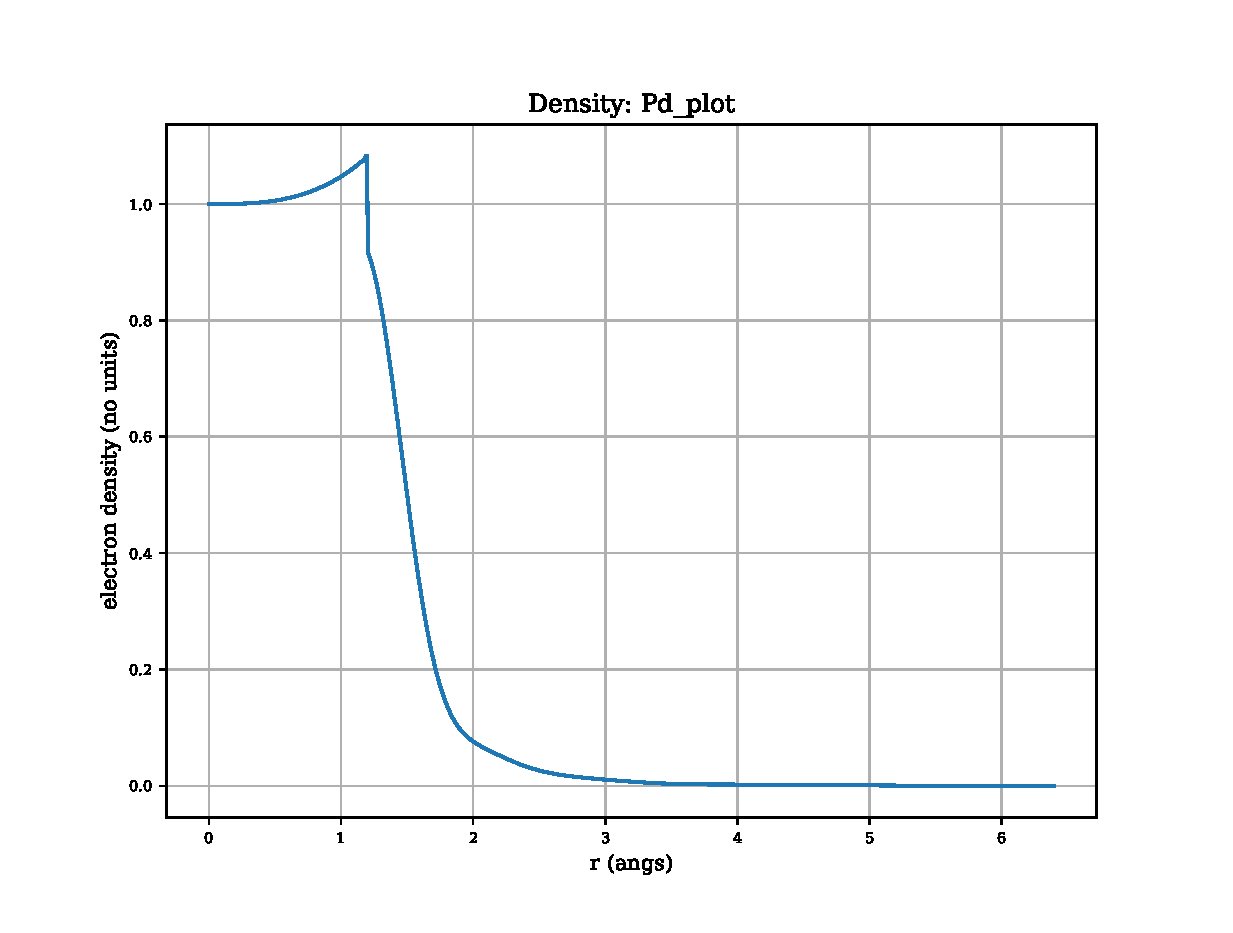
\includegraphics[width=\linewidth]{chapters/potentials_fe_pd_ru/sheng/Pd_plot_den.eps}
\caption{Sheng palladium density function}
\label{fig:shengpddens}
\endminipage\hfill
\minipage{0.49\textwidth}
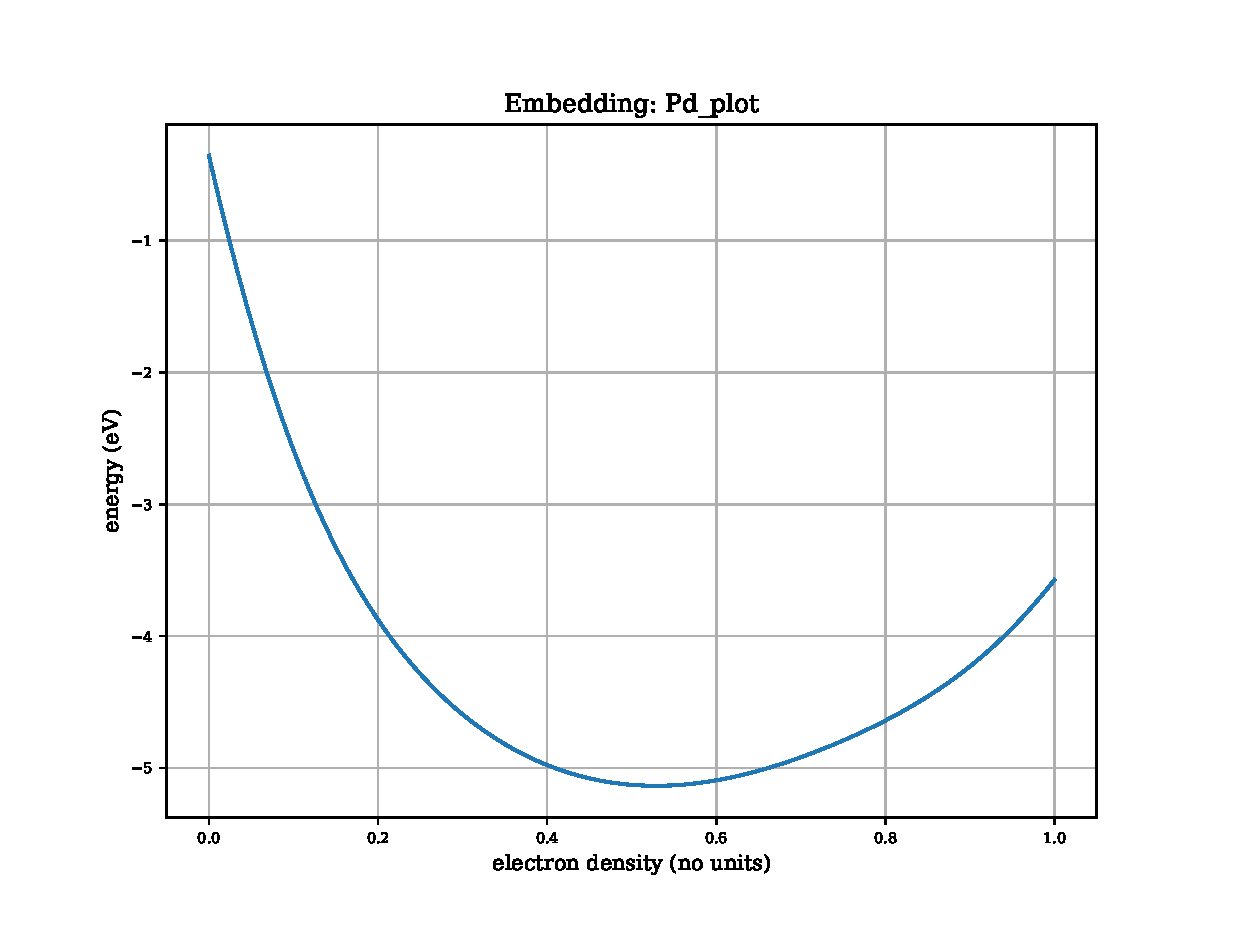
\includegraphics[width=\linewidth]{chapters/potentials_fe_pd_ru/sheng/Pd_plot_embed.eps}
\caption{Sheng palladium embedding function}
\label{fig:shengpdembe}
\endminipage
\end{figure}

\FloatBarrier


\end{comment}
